\documentclass[a4paper,11pt]{article}

\newcommand{\triposcourse}{Markov Chains}
\usepackage{fancyhdr,titlesec,geometry}
\usepackage[dvipsnames]{xcolor}
\usepackage[many]{tcolorbox}
\usepackage{xifthen}
\usepackage{import}
\usepackage{parskip}
\usepackage{transparent}
\usepackage{mathtools,amssymb,amsfonts,amsthm,bm}   % Math Presets
\usepackage{array,tabularx,booktabs}                % Table Presets
\usepackage{graphicx,wrapfig,float,caption}         % Figure Presets
\usepackage{setspace,multicol}                      % Text Presets
\usepackage{tikz,physics,cancel,tkz-euclide,pgfplots,tikz-3dplot}                    % Physics Presets
\usepackage{amsmath}
\usepackage{mathrsfs}
\usepackage{enumerate}
\usepackage[shortlabels]{enumitem}
\usepackage{hyperref}
\usepackage{lipsum}
\usepackage{IEEEtrantools}
\usepackage{xcomment}
\usepackage{sectsty}
\usepackage{thmtools}
\usepackage{mdframed}
\usepackage{siunitx}
\usepackage{centernot}

\newcommand{\sectionbreak}{\clearpage}

\tdplotsetmaincoords{60}{120}

\usetikzlibrary{arrows.meta}
\usetikzlibrary{decorations.markings}
\usetikzlibrary{decorations.pathmorphing}
\usetikzlibrary{automata, positioning}
\usetikzlibrary{fadings}
\usetikzlibrary{intersections}
\usetikzlibrary{cd}
\usetikzlibrary{patterns}
\usetikzlibrary{shapes.arrows}
\usepgfplotslibrary{colormaps, external}
\pgfarrowsdeclarecombine{twolatex'}{twolatex'}{latex'}{latex'}{latex'}{latex'}
\tikzset{->/.style = {decoration={markings,
                                  mark=at position 1 with {\arrow[scale=1.6]{latex'}}},
                      postaction={decorate}}}
\tikzset{<-/.style = {decoration={markings,
                                  mark=at position 0 with {\arrowreversed[scale=1.6]{latex'}}},
                      postaction={decorate}}}
\tikzset{<->/.style = {decoration={markings,
                                   mark=at position 0 with {\arrowreversed[scale=1.6]{latex'}},
                                   mark=at position 1 with {\arrow[scale=1.6]{latex'}}},
                       postaction={decorate}}}
\tikzset{->-/.style = {decoration={markings,
                                   mark=at position #1 with {\arrow[scale=1.6]{latex'}}},
                       postaction={decorate}}}
\tikzset{-<-/.style = {decoration={markings,
                                   mark=at position #1 with {\arrowreversed[scale=1.6]{latex'}}},
                       postaction={decorate}}}
\tikzset{->>/.style = {decoration={markings,
                                  mark=at position 1 with {\arrow[scale=1.6]{twolatex'}}},
                      postaction={decorate}}}
\tikzset{<<-/.style = {decoration={markings,
                                  mark=at position 0 with {\arrowreversed[scale=1.6]{twolatex'}}},
                      postaction={decorate}}}
\tikzset{<<->>/.style = {decoration={markings,
                                   mark=at position 0 with {\arrowreversed[scale=1.6]{twolatex'}},
                                   mark=at position 1 with {\arrow[scale=1.6]{twolatex'}}},
                       postaction={decorate}}}
\tikzset{->>-/.style = {decoration={markings,
                                   mark=at position #1 with {\arrow[scale=1.6]{twolatex'}}},
                       postaction={decorate}}}
\tikzset{-<<-/.style = {decoration={markings,
                                   mark=at position #1 with {\arrowreversed[scale=1.6]{twolatex'}}},
                       postaction={decorate}}}

\tikzset{
set arrow inside/.code={\pgfqkeys{/tikz/arrow inside}{#1}},
set arrow inside={end/.initial=>, opt/.initial=},
/pgf/decoration/Mark/.style={
    mark/.expanded=at position #1 with
    {
        \noexpand\arrow[\pgfkeysvalueof{/tikz/arrow inside/opt}]{\pgfkeysvalueof{/tikz/arrow inside/end}}
    }
},
arrow inside/.style 2 args={
    set arrow inside={#1},
    postaction={
        decorate,decoration={
            markings,Mark/.list={#2}
        }
    }
},
}

\tikzstyle{circ}=[fill=black, draw=black, shape=circle]
\tikzset{
dot/.style = {circle, fill, minimum size=#1,
              inner sep=0pt, outer sep=0pt},
dot/.default = 5pt% size of the circle diameter 
}
\tikzset{mstate/.style={circle, draw, blue, text=black, minimum width=0.7cm}}
\tikzset{snake it/.style={-stealth,
decoration={snake, 
    amplitude = .4mm,
    segment length = 2mm,
    post length=0.9mm},decorate}}

\def\centerarc[#1](#2)(#3:#4:#5)% Syntax: [draw options](center)(initial angle:final angle:radius)
    { \draw[#1] ($(#2)+({#5*cos(#3)},{#5*sin(#3)})$) arc (#3:#4:#5); }

\hypersetup{
    colorlinks=true,
    linkcolor=blue,
    filecolor=blue,
    citecolor = black,      
    urlcolor=cyan,
    }

%%%%%%%%%%% Snippets %%%%%%%%%%%%%%%%
\newcommand*\widefbox[1]{\fbox{\hspace{2em}#1\hspace{2em}}}
\newcommand{\xint}{\int_{x_1}^{x_2}}
\newcommand{\mw}{\sqrt{m\omega}}
\newcommand{\de}{\delta}
\newcommand{\dde}{\dot{\delta}}
\newcommand{\di}{\delta_i}
\newcommand{\ddi}{\dot{\delta_i}}
\newcommand{\dddi}{\ddot{\delta_i}}
\newcommand{\dipl}{\delta_{i+1}}
\newcommand{\dimi}{\delta_{i-1}}
\newcommand{\ddt}[1]{\frac{{d} #1}{dt}}
\newcommand{\ddtt}[1]{\frac{d^2 #1}{dt^2}}
\newcommand{\ddx}[1]{\frac{d #1}{dx}}
\newcommand{\ddxx}[1]{\frac{d^2 #1}{dx^2}}
\newcommand{\eps}{\epsilon}
\newcommand{\del}[2]{\frac{\partial #1}{\partial #2}}
\newcommand{\deltwo}[2]{\frac{\partial^2 #1}{\partial #2^2}}
\newcommand{\lam}{\lambda}
\newcommand{\Lam}{\Lambda}
\newcommand{\sig}{\sigma}
\newcommand{\Sig}{\Sigma}
\newcommand{\half}{\frac{1}{2}}
\newcommand{\munu}{{\mu\nu}}
\newcommand{\thalf}{\tfrac{1}{2}}
\renewcommand{\div}{\nabla\cdot}
\renewcommand{\curl}{\nabla\times}

\DeclareMathOperator{\orb}{Orb}
\DeclareMathOperator{\stab}{Stab}
\DeclareMathOperator{\adj}{adj}
\DeclareMathOperator{\ccl}{ccl}
\let\var\relax
\DeclareMathOperator{\var}{Var}
\DeclareMathOperator{\cov}{Cov}
\DeclareMathOperator{\corr}{Corr}
\DeclareMathOperator{\Markov}{Markov}
\DeclareMathOperator{\nullity}{nullity}

\newcommand{\bfA}{{\bf A}}
\newcommand{\bfB}{{\bf B}}
\newcommand{\bfC}{{\bf C}}
\newcommand{\bfD}{{\bf D}}
\newcommand{\bfE}{{\bf E}}
\newcommand{\bfF}{{\bf F}}
\newcommand{\bfG}{{\bf G}}
\newcommand{\bfH}{{\bf H}}
\newcommand{\bfI}{{\bf I}}
\newcommand{\bfJ}{{\bf J}}
\newcommand{\bfK}{{\bf K}}
\newcommand{\bfL}{{\bf L}}
\newcommand{\bfM}{{\bf M}}
\newcommand{\bfN}{{\bf N}}
\newcommand{\bfO}{{\bf O}}
\newcommand{\bfP}{{\bf P}}
\newcommand{\bfQ}{{\bf Q}}
\newcommand{\bfR}{{\bf R}}
\newcommand{\bfS}{{\bf S}}
\newcommand{\bfT}{{\bf T}}
\newcommand{\bfU}{{\bf U}}
\newcommand{\bfV}{{\bf V}}
\newcommand{\bfW}{{\bf W}}
\newcommand{\bfX}{{\bf X}}
\newcommand{\bfY}{{\bf Y}}
\newcommand{\bfZ}{{\bf Z}}

\newcommand{\bfa}{{\bf a}}
\newcommand{\bfb}{{\bf b}}
\newcommand{\bfc}{{\bf c}}
\newcommand{\bfd}{{\bf d}}
\newcommand{\bfe}{{\bf e}}
\newcommand{\bff}{{\bf f}}
\newcommand{\bfg}{{\bf g}}
\newcommand{\bfh}{{\bf h}}
\newcommand{\bfi}{{\bf i}}
\newcommand{\bfj}{{\bf j}}
\newcommand{\bfk}{{\bf k}}
\newcommand{\bfl}{{\bf l}}
\newcommand{\bfm}{{\bf m}}
\newcommand{\bfn}{{\bf n}}
\newcommand{\bfo}{{\bf o}}
\newcommand{\bfp}{{\bf p}}
\newcommand{\bfq}{{\bf q}}
\newcommand{\bfr}{{\bf r}}
\newcommand{\bfs}{{\bf s}}
\newcommand{\bft}{{\bf t}}
\newcommand{\bfu}{{\bf u}}
\newcommand{\bfv}{{\bf v}}
\newcommand{\bfw}{{\bf w}}
\newcommand{\bfx}{{\bf x}}
\newcommand{\bfy}{{\bf y}}
\newcommand{\bfz}{{\bf z}}

\newcommand{\mcA}{{\mathcal{A}}}
\newcommand{\mcB}{{\mathcal{B}}}
\newcommand{\mcC}{{\mathcal{C}}}
\newcommand{\mcD}{{\mathcal{D}}}
\newcommand{\mcE}{{\mathcal{E}}}
\newcommand{\mcF}{{\mathcal{F}}}
\newcommand{\mcG}{{\mathcal{G}}}
\newcommand{\mcH}{{\mathcal{H}}}
\newcommand{\mcI}{{\mathcal{I}}}
\newcommand{\mcJ}{{\mathcal{J}}}
\newcommand{\mcK}{{\mathcal{K}}}
\newcommand{\mcL}{{\mathcal{L}}}
\newcommand{\mcM}{{\mathcal{M}}}
\newcommand{\mcN}{{\mathcal{N}}}
\newcommand{\mcO}{{\mathcal{O}}}
\newcommand{\mcP}{{\mathcal{P}}}
\newcommand{\mcQ}{{\mathcal{Q}}}
\newcommand{\mcR}{{\mathcal{R}}}
\newcommand{\mcS}{{\mathcal{S}}}
\newcommand{\mcT}{{\mathcal{T}}}
\newcommand{\mcU}{{\mathcal{U}}}
\newcommand{\mcV}{{\mathcal{V}}}
\newcommand{\mcW}{{\mathcal{W}}}
\newcommand{\mcX}{{\mathcal{X}}}
\newcommand{\mcY}{{\mathcal{Y}}}
\newcommand{\mcZ}{{\mathcal{Z}}}

\newcommand{\bbA}{{\mathbb{A}}}
\newcommand{\bbB}{{\mathbb{B}}}
\newcommand{\bbC}{{\mathbb{C}}}
\newcommand{\bbD}{{\mathbb{D}}}
\newcommand{\bbE}{{\mathbb{E}}}
\newcommand{\bbF}{{\mathbb{F}}}
\newcommand{\bbG}{{\mathbb{G}}}
\newcommand{\bbH}{{\mathbb{H}}}
\newcommand{\bbI}{{\mathbb{I}}}
\newcommand{\bbJ}{{\mathbb{J}}}
\newcommand{\bbK}{{\mathbb{K}}}
\newcommand{\bbL}{{\mathbb{L}}}
\newcommand{\bbM}{{\mathbb{M}}}
\newcommand{\bbN}{{\mathbb{N}}}
\newcommand{\bbO}{{\mathbb{O}}}
\newcommand{\bbP}{{\mathbb{P}}}
\newcommand{\bbQ}{{\mathbb{Q}}}
\newcommand{\bbR}{{\mathbb{R}}}
\newcommand{\bbS}{{\mathbb{S}}}
\newcommand{\bbT}{{\mathbb{T}}}
\newcommand{\bbU}{{\mathbb{U}}}
\newcommand{\bbV}{{\mathbb{V}}}
\newcommand{\bbW}{{\mathbb{W}}}
\newcommand{\bbX}{{\mathbb{X}}}
\newcommand{\bbY}{{\mathbb{Y}}}
\newcommand{\bbZ}{{\mathbb{Z}}}

\newcommand{\mfa}{{\mathfrak{a}}}
\newcommand{\mfb}{{\mathfrak{b}}}
\newcommand{\mfc}{{\mathfrak{c}}}
\newcommand{\mfd}{{\mathfrak{d}}}
\newcommand{\mfe}{{\mathfrak{e}}}
\newcommand{\mff}{{\mathfrak{f}}}
\newcommand{\mfg}{{\mathfrak{g}}}
\newcommand{\mfh}{{\mathfrak{h}}}
\newcommand{\mfi}{{\mathfrak{i}}}
\newcommand{\mfj}{{\mathfrak{j}}}
\newcommand{\mfk}{{\mathfrak{k}}}
\newcommand{\mfl}{{\mathfrak{l}}}
\newcommand{\mfm}{{\mathfrak{m}}}
\newcommand{\mfn}{{\mathfrak{n}}}
\newcommand{\mfo}{{\mathfrak{o}}}
\newcommand{\mfp}{{\mathfrak{p}}}
\newcommand{\mfq}{{\mathfrak{q}}}
\newcommand{\mfr}{{\mathfrak{r}}}
\newcommand{\mfs}{{\mathfrak{s}}}
\newcommand{\mft}{{\mathfrak{t}}}
\newcommand{\mfu}{{\mathfrak{u}}}
\newcommand{\mfv}{{\mathfrak{v}}}
\newcommand{\mfw}{{\mathfrak{w}}}
\newcommand{\mfx}{{\mathfrak{x}}}
\newcommand{\mfy}{{\mathfrak{y}}}
\newcommand{\mfz}{{\mathfrak{z}}}

\newcommand{\mfA}{{\mathfrak{A}}}
\newcommand{\mfB}{{\mathfrak{B}}}
\newcommand{\mfC}{{\mathfrak{C}}}
\newcommand{\mfD}{{\mathfrak{D}}}
\newcommand{\mfE}{{\mathfrak{E}}}
\newcommand{\mfF}{{\mathfrak{F}}}
\newcommand{\mfG}{{\mathfrak{G}}}
\newcommand{\mfH}{{\mathfrak{H}}}
\newcommand{\mfI}{{\mathfrak{I}}}
\newcommand{\mfJ}{{\mathfrak{J}}}
\newcommand{\mfK}{{\mathfrak{K}}}
\newcommand{\mfL}{{\mathfrak{L}}}
\newcommand{\mfM}{{\mathfrak{M}}}
\newcommand{\mfN}{{\mathfrak{N}}}
\newcommand{\mfO}{{\mathfrak{O}}}
\newcommand{\mfP}{{\mathfrak{P}}}
\newcommand{\mfQ}{{\mathfrak{Q}}}
\newcommand{\mfR}{{\mathfrak{R}}}
\newcommand{\mfS}{{\mathfrak{S}}}
\newcommand{\mfT}{{\mathfrak{T}}}
\newcommand{\mfU}{{\mathfrak{U}}}
\newcommand{\mfV}{{\mathfrak{V}}}
\newcommand{\mfW}{{\mathfrak{W}}}
\newcommand{\mfX}{{\mathfrak{X}}}
\newcommand{\mfY}{{\mathfrak{Y}}}
\newcommand{\mfZ}{{\mathfrak{Z}}}

\newcommand{\rma}{\mathrm{a}}
\newcommand{\rmb}{\mathrm{b}}
\newcommand{\rmc}{\mathrm{c}}
\newcommand{\rmd}{\mathrm{d}}
\renewcommand{\dd}{\,\mathrm{d}}
\newcommand{\rme}{\mathrm{e}}
\newcommand{\rmf}{\mathrm{f}}
\newcommand{\rmg}{\mathrm{g}}
\newcommand{\rmh}{\mathrm{h}}
\newcommand{\rmi}{\mathrm{i}}
\newcommand{\rmj}{\mathrm{j}}
\newcommand{\rmk}{\mathrm{k}}
\newcommand{\rml}{\mathrm{l}}
\newcommand{\rmm}{\mathrm{m}}
\newcommand{\rmn}{\mathrm{n}}
\newcommand{\rmo}{\mathrm{o}}
\newcommand{\rmp}{\mathrm{p}}
\newcommand{\rmq}{\mathrm{q}}
\newcommand{\rmr}{\mathrm{r}}
\newcommand{\rms}{\mathrm{s}}
\newcommand{\rmt}{\mathrm{t}}
\newcommand{\rmu}{\mathrm{u}}
\newcommand{\rmv}{\mathrm{v}}
\newcommand{\rmw}{\mathrm{w}}
\newcommand{\rmx}{\mathrm{x}}
\newcommand{\rmy}{\mathrm{y}}
\newcommand{\rmz}{\mathrm{z}}
\newcommand{\rmA}{\mathrm{A}}
\newcommand{\rmB}{\mathrm{B}}
\newcommand{\rmC}{\mathrm{C}}
\newcommand{\rmD}{\mathrm{D}}
\newcommand{\rmE}{\mathrm{E}}
\newcommand{\rmF}{\mathrm{F}}
\newcommand{\rmG}{\mathrm{G}}
\newcommand{\rmH}{\mathrm{H}}
\newcommand{\rmI}{\mathrm{I}}
\newcommand{\rmJ}{\mathrm{J}}
\newcommand{\rmK}{\mathrm{K}}
\newcommand{\rmL}{\mathrm{L}}
\newcommand{\rmM}{\mathrm{M}}
\newcommand{\rmN}{\mathrm{N}}
\newcommand{\rmO}{\mathrm{O}}
\newcommand{\rmP}{\mathrm{P}}
\newcommand{\rmQ}{\mathrm{Q}}
\newcommand{\rmR}{\mathrm{R}}
\newcommand{\rmS}{\mathrm{S}}
\newcommand{\rmT}{\mathrm{T}}
\newcommand{\rmU}{\mathrm{U}}
\newcommand{\rmV}{\mathrm{V}}
\newcommand{\rmW}{\mathrm{W}}
\newcommand{\rmX}{\mathrm{X}}
\newcommand{\rmY}{\mathrm{Y}}
\newcommand{\rmZ}{\mathrm{Z}}

\newcommand{\GL}{\mathrm{GL}}
\newcommand{\Or}{\mathrm{O}}
\newcommand{\PGL}{\mathrm{PGL}}
\newcommand{\PSL}{\mathrm{PSL}}
\newcommand{\PSO}{\mathrm{PSO}}
\newcommand{\PSU}{\mathrm{PSU}}
\newcommand{\SL}{\mathrm{SL}}
\newcommand{\SO}{\mathrm{SO}}
\newcommand{\Spin}{\mathrm{Spin}}
\newcommand{\Sp}{\mathrm{Sp}}
\newcommand{\SU}{\mathrm{SU}}
\newcommand{\Mat}{\mathrm{Mat}}

% Some common notations

\renewcommand{\v}{\mathbf{v}}
\newcommand{\w}{\mathbf{w}}
\renewcommand{\u}{\mathbf{u}}

% Matrix algebras
\newcommand{\gl}{\mathfrak{gl}}
\newcommand{\ort}{\mathfrak{o}}
\newcommand{\so}{\mathfrak{so}}
\newcommand{\su}{\mathfrak{su}}
\newcommand{\uu}{\mathfrak{u}}
\renewcommand{\sl}{\mathfrak{sl}}
\newcommand{\inner}[1]{\left\langle{#1}\right\rangle}
\DeclareMathOperator{\spn}{span}

\newcommand{\mobius}{{M\"{o}bius }}

\renewcommand{\ge}{\geqslant}
\renewcommand{\le}{\leqslant}
\renewcommand{\geq}{\geqslant}
\renewcommand{\leq}{\leqslant}
\renewcommand{\restriction}{\mathord{\upharpoonright}}

\newcommand\independent{\protect\mathpalette{\protect\independenT}{\perp}}
\def\independenT#1#2{\mathrel{\rlap{$#1#2$}\mkern2mu{#1#2}}}

\setlength{\parindent}{0pt}
% \setlength{\parskip}{\baselineskip}
\newcommand{\incfig}[1]{%
    \def\svgwidth{0.4\columnwidth}
    \import{./figures/}{#1.pdf_tex}
}
%%%%%%%%%%%%%%%%%%%%%%%%%%%%%%%%%%%%%

\usepackage[T1]{fontenc}
\usepackage{lmodern,mathrsfs}

%%%%%%%boxed enviroment for final layout%%%%%%%%%%%%%

\newtheoremstyle{mystyle}%
  {}%
  {}%
  {}%
  {}%
  {\sffamily\bfseries}%
  {.}%
  { }%
  {}%

% \renewenvironment{proof}{{\sffamily\bfseries Proof. }}{\qed}

\theoremstyle{mystyle}{
  \newtheorem{theorem}{Theorem}[section]
  \newtheorem{lemma}[theorem]{Lemma}
  \newtheorem{proposition}[theorem]{Proposition}
  \newtheorem{corollary}[theorem]{Corollary}
  \newtheorem{problem}[theorem]{Problem}
  \newtheorem*{claim}{Claim}
  \newtheorem*{slemma}{Lemma}
  \newtheorem*{sprop}{Proposition}
  \newtheorem*{notation}{Notation}

  \newtheorem{inquestion}{Question}
  \newtheorem*{sque}{Question}

  \newtheorem{definition}{Definition}[section]
  \newtheorem{conjecture}{Conjecture}[section]
  \newtheorem{example}{Example}[section]
  \newtheorem*{law}{Law}

  \newtheorem*{remark}{Remark}
  \newtheorem*{note}{Note}
}

\newenvironment{question}[1]
{\renewcommand\theinquestion{#1}\inquestion}
{\endinquestion}

\theoremstyle{definition}{
    \newtheorem*{exercise}{Exercise}}

\tcolorboxenvironment{definition}{
  boxrule=0pt,
  boxsep=2pt,
  colback={White!90!Cerulean},
  enhanced jigsaw, 
  borderline west={2pt}{0pt}{Cerulean},
  sharp corners,
  before skip=10pt,
  after skip=10pt,
  breakable,
  % parbox=false,
}

\tcolorboxenvironment{notation}{
  boxrule=0pt,
  boxsep=2pt,
  colback={White!90!Cerulean},
  enhanced jigsaw, 
  borderline west={2pt}{0pt}{Cerulean},
  sharp corners,
  before skip=10pt,
  after skip=10pt,
  breakable,
  % parbox=false,
}

\tcolorboxenvironment{proposition}{
  boxrule=0pt,
  boxsep=2pt,
  colback={White!90!Yellow},
  enhanced jigsaw, 
  borderline west={2pt}{0pt}{Yellow},
  sharp corners,
  before skip=10pt,
  after skip=10pt,
  breakable,
  % parbox=false,
}

\tcolorboxenvironment{sprop}{
  boxrule=0pt,
  boxsep=2pt,
  colback={White!90!Yellow},
  enhanced jigsaw, 
  borderline west={2pt}{0pt}{Yellow},
  sharp corners,
  before skip=10pt,
  after skip=10pt,
  breakable,
  % parbox=false,
}

\tcolorboxenvironment{theorem}{
  boxrule=0pt,
  boxsep=2pt,
  colback={White!90!Dandelion},
  enhanced jigsaw, 
  borderline west={2pt}{0pt}{Dandelion},
  sharp corners,
  before skip=10pt,
  after skip=10pt,
  breakable,
  % parbox=false,
}

\tcolorboxenvironment{lemma}{
  boxrule=0pt,
  boxsep=2pt,
  blanker,
  borderline west={2pt}{0pt}{Red},
  before skip=10pt,
  after skip=10pt,
  sharp corners,
  left=12pt,
  right=12pt,
  breakable,
  % parbox=false,
}

\tcolorboxenvironment{corollary}{
  boxrule=0pt,
  boxsep=2pt,
  blanker,
  borderline west={2pt}{0pt}{ForestGreen},
  before skip=10pt,
  after skip=10pt,
  sharp corners,
  left=12pt,
  right=12pt,
  breakable,
  % parbox=false,
}

\tcolorboxenvironment{proof}{
  boxrule=0pt,
  boxsep=2pt,
  blanker,
  borderline west={2pt}{0pt}{NavyBlue!80!white},
  before skip=10pt,
  after skip=10pt,
  left=12pt,
  right=12pt,
  breakable,
  % parbox=false,
}

\tcolorboxenvironment{remark}{
  boxrule=0pt,
  boxsep=2pt,
  blanker,
  borderline west={2pt}{0pt}{Green},
  before skip=10pt,
  after skip=10pt,
  left=12pt,
  right=12pt,
  breakable,
  % parbox=false,
}

\tcolorboxenvironment{note}{
  boxrule=0pt,
  boxsep=2pt,
  blanker,
  borderline west={2pt}{0pt}{PineGreen},
  before skip=10pt,
  after skip=10pt,
  left=12pt,
  right=12pt,
  breakable,
  % parbox=false,
}

\tcolorboxenvironment{example}{
  boxrule=0pt,
  boxsep=2pt,
  blanker,
  borderline west={2pt}{0pt}{Black},
  sharp corners,
  before skip=10pt,
  after skip=10pt,
  left=12pt,
  right=12pt,
  breakable,
  % parbox=false,
}

\titleformat*{\section}{\Large\bfseries\sffamily}
\titleformat*{\subsection}{\large\bfseries\sffamily}
\titleformat*{\subsubsection}{\bfseries\sffamily}
\titleformat*{\paragraph}{\bfseries\sffamily}

%%%%%%%%%%%%%%%%%%%%%%%%%%%%%%%%%%%%%%%%%%%%%%%%%%%%

\title{\textbf{\sffamily\triposcourse{} Notes}}
% \usepackage[T1]{fontenc}
\usepackage{crimson}

\theoremstyle{plain}

\theoremstyle{definition}
\newtheorem{theorem}{Theorem}[section]
\newtheorem{lemma}[theorem]{Lemma}
\newtheorem{proposition}[theorem]{Proposition}
\newtheorem{corollary}[theorem]{Corollary}
\newtheorem{problem}[theorem]{Problem}
\newtheorem*{claim}{Claim}
\newtheorem*{slemma}{Lemma}
\newtheorem*{sprop}{Proposition}
\newtheorem*{notation}{Notation}
\newtheorem*{exercise}{Exercise}

\newtheorem{inquestion}{Question}
\newtheorem*{sque}{Question}
\newenvironment{question}[1]
  {\renewcommand\theinquestion{#1}\inquestion}
  {\endinquestion}

\newtheorem{definition}{Definition}[section]
\newtheorem{conjecture}{Conjecture}[section]
\newtheorem{example}{Example}[section]
\newtheorem*{law}{Law}

\theoremstyle{remark}
\newtheorem*{remark}{Remark}
\newtheorem*{note}{Note}

\title{\textbf{\triposcourse{} Notes}}
% \theoremstyle{plain}{
  \newtheorem{theorem}{Theorem}[section]
  \newtheorem{lemma}[theorem]{Lemma}
  \newtheorem{proposition}[theorem]{Proposition}
  \newtheorem{corollary}[theorem]{Corollary}
  \newtheorem*{claim}{Claim}
  \newtheorem*{slemma}{Lemma}
  \newtheorem*{sprop}{Proposition}
  \newtheorem{conjecture}{Conjecture}[section]
  \newtheorem*{law}{Law}
  \newtheorem{inquestion}{Question}
  \newtheorem*{sque}{Question}
}

\theoremstyle{definition}{
  \newtheorem{method}[theorem]{Method}
  \newtheorem{definition}{Definition}[section]
  \newtheorem{example}{Example}[section]
  \newtheorem*{notation}{Notation}
  \newtheorem*{exercise}{Exercise}
}

\theoremstyle{remark}{
  \newtheorem{remark}[theorem]{Remark}
  \newtheorem*{note}{Note}
}

\newenvironment{question}[1]
{\renewcommand\theinquestion{#1}\inquestion}
{\endinquestion}

\title{\textbf{\sffamily\triposcourse{} Notes}}

%layout full
% \geometry{%
%   a4paper,
%   lmargin=2cm,
%   rmargin=2.5cm,
%   tmargin=3.5cm,
%   bmargin=2.5cm,
%   footskip=12pt,
%   headheight=24pt}
% layout trim
% \geometry{
% papersize={379pt, 542pt},
% textwidth=345pt,
% textheight=443pt,
% left=17pt,
% top=54pt,
% right=17pt
% }
% layout a5
\geometry{%
  a5paper,
  lmargin=1cm,
  rmargin=1cm,
  tmargin=2.5cm,
  bmargin=1.5cm,
  footskip=15pt,
  headheight=24pt}
\pagestyle{fancy}
\rhead{{\triposcourse{}}}
\author{jt775}
\AddToHook{cmd/section/before}{\clearpage}

\graphicspath{ {./images/} }
\pgfplotsset{compat=1.17}
\begin{document}
\maketitle
\clearpage
\tableofcontents
\clearpage 

\section{Definition of a Markov chain}
Throughout the note, let $ I $ be a finite or countable set, and any random variables will be defined on the same probability space $ (\Omega, \mathcal{F}, \mathbb{P}) $.

\begin{definition}[Markov Chains]
    A stochastic process $ X=(X_n)_{n\ge 0} $ is called a \textbf{Markov chain} if $ \forall n\ge 0 $ and for all $ x_1,\dots,x_n\in I $, we have 
    \[
        \begin{aligned}
            &\mathbb{P}(X_{n+1}=x_{n+1}|X_n=x_n, X_{n-1}=x_{n-1}, \dots, X_0=x_0)\\ &= \mathbb{P}(X_{n+1}=x_{n+1}|X_n=x_n).
        \end{aligned}
    \]
\end{definition}
\begin{definition}[Time-homogeneous]
    A Markov chain $X$ is called \textbf{time} \textbf{homogeneous} if $ \mathbb{P}(X_{n+1}=y|X_n=x),\ \forall x,y\in I $ is independent of $n$. Otherwise it is called \textbf{time-inhomogeneous}.
\end{definition}
We will only be dealing with time-homogeneous Markov chains in this course.
\begin{definition}[Stochastic matrix]
    A matrix $P$ is called a \textbf{stochastic matrix} if $ \sum_{y}P(x,y)=1 $.
\end{definition}

\begin{definition}[Transitional matrix]
    $P$ be a matrix such that $ P(x,y) = \mathbb{P}(X_1=y|X_0=x), x,y\in I $. $P$ is called the \textbf{transitional matrix} of $X$.
\end{definition}

We see that $P$ is a stochastic matrix.

\begin{remark}
    \begin{enumerate}
        \item The index set of a markov chain needs not to be $\bbN$. It could be $ \{1,\dots,N\} $, where $ N\in \mathbb{N} $.
        \item Since $X$ is time-homogeneous, $ P(x,y)=\mathbb{P}(X_1=y|X_0=x)=\mathbb{P}(X_{n+1}=y|X_n=x) $ for all $n$.
    \end{enumerate}
\end{remark}

\begin{definition}
    We say that $X$ is $ \Markov(\lambda,P) $ if $ X_0 $ has distribution $\lambda$ and $ P $ is the transitional matrix of $X$, i.e. 
    \begin{enumerate}[(i)]
        \item $ \mathbb{P}(X_0=x_0)=\lambda_{x_0},\ \forall x_0\in I $,
        \item $ \mathbb{P}(X_{n+1}=x_{n+1}|X_n=x_n, X_{n-1}=x_{n-1}, \dots, X_0=x_0) = P(x_{n},x_{n+1}) $.
    \end{enumerate}
\end{definition}
\begin{note}
    We also write $ P(x,y)=P_{xy} $.
\end{note}

We usually represent a Markov chain by its \textit{diagram} corresponding to the allowed transitions.
\begin{example}
    Let $ \alpha,\beta\in (0,1) $ and consider 
    \[
        P = \begin{pmatrix}
            \alpha & 1-\alpha \\
            1-\beta & \beta \\
        \end{pmatrix}.
    \]
    The diagram is as follows:
    \begin{center}
        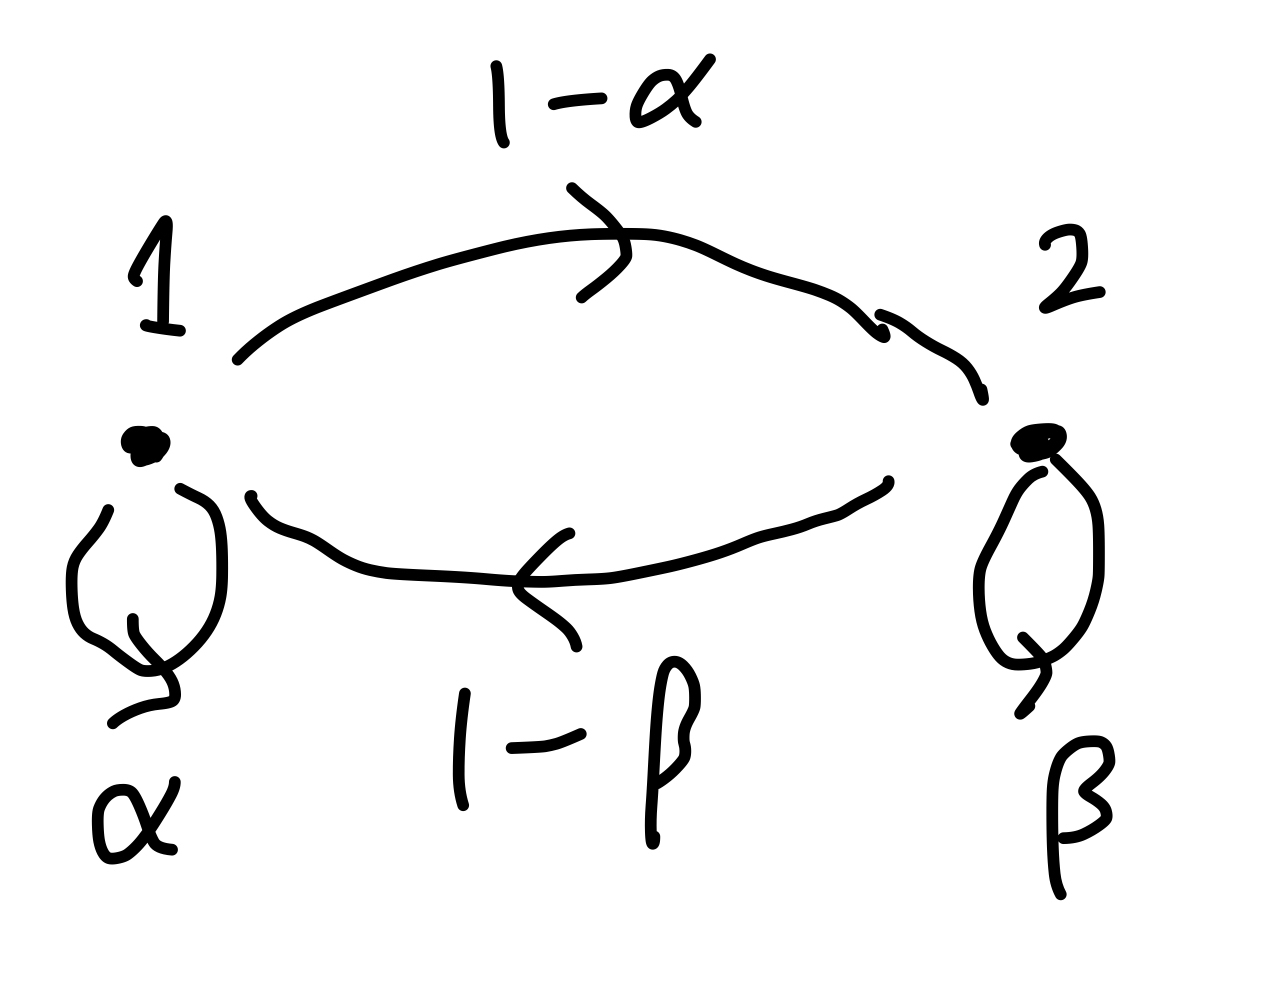
\includegraphics[scale=0.07]{markov1.jpeg}
    \end{center}
\end{example}

\begin{example}
    Let $ P = \begin{pmatrix}
        1/2 & 1/2 & 0 \\
        1/3 & 1/3 & 1/3 \\
        1 & 0 & 0 \\
    \end{pmatrix} $. The diagram is
    \begin{center}
        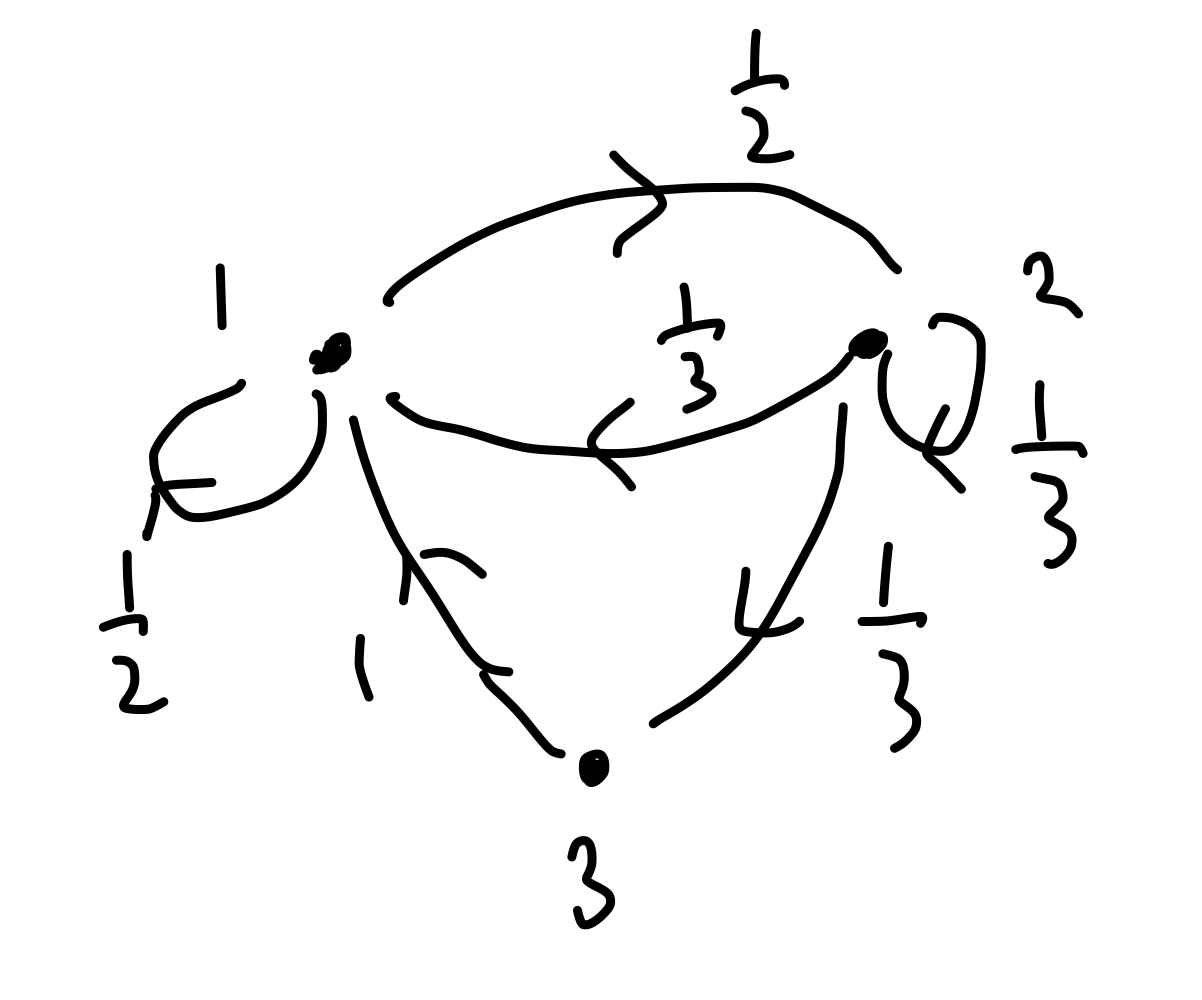
\includegraphics[scale=0.09]{markov2.jpeg}
    \end{center}
\end{example}

\section{Basic properties}

The next theorem gives the condition for $X$ to be Markov.

\begin{theorem}\label{thm:1.1}
    The process $X$ is $ \Markov(\lambda,P) $ if and only if $ \forall n\ge 0 $ and for all $ x_0,\dots,x_n\in I $, we have 
    \[
        \mathbb{P}(X_0=x_0,\dots,X_n=x_n) = \lambda_{x_0} P(x_0,x_1)\cdots P(x_{n-1},x_n).
    \]
\end{theorem}
\begin{proof}
    Suppose $ X $ is $ \Markov(\lambda,P) $. Then 
    \begin{align*}
        &\mathbb{P}(X_0=x_0,\dots,X_n=x_n)\\ &= \mathbb{P}(X_n=x_n,X_{n-1}=x_{n-1},\dots, X_0=x_0|X_{n-1}=x_{n-1},\dots, X_0=x_0)\\
        &\quad\cdot \mathbb{P}(X_{n-1}=x_{n-1},\dots, X_0=x_0 )\\
        &= \mathbb{P}(X_n=x_n|X_{n-1}=x_{n-1},\dots, X_0=x_0)\mathbb{P}(X_{n-1}=x_{n-1},\dots, X_0=x_0 )\\ 
        &= P(x_{n-1},x_n)\mathbb{P}(X_{n-1}=x_{n-1},\dots, X_0=x_0 )\\ 
        &=\cdots\\ 
        &= \mathbb{P}(X_0=x_0) P(x_0,x_1)\cdots P(x_{n-1},x_n)\\ 
        &= \lambda_{x_0} P(x_0,x_1)\cdots P(x_{n-1},x_n).
    \end{align*}

    Suppose conversely that $ \forall n\ge 0 $ and for all $ x_0,\dots,x_n\in I $, we have 
    \[
        \mathbb{P}(X_0=x_0,\dots,X_n=x_n) = \lambda_{x_0} P(x_0,x_1)\cdots P(x_{n-1},x_n).
    \]
    Setting $n=0$ gives $ \mathbb{P}(X_0=x_0)=\lambda_{x_0} $. By definition, consider 
    \begin{align*}
        &\mathbb{P}(X_n=x_n|X_{n-1}=x_{n-1},\dots, X_0=x_0)\\ &= \frac{\mathbb{P}(X_0=x_0,\dots,X_n=x_n)}{\mathbb{P}(X_0=x_0,\dots,X_{n-1}=x_{n-1})}\\ 
        &= \frac{\lambda_{x_0} P(x_0,x_1)\cdots P(x_{n-1},x_n)}{\lambda_{x_0} P(x_0,x_1)\cdots P(x_{n-2},x_{n-1})}\\ 
        &= P(x_{n-1},x_n).\qedhere
    \end{align*}
\end{proof}

\begin{definition}
    For $i\in I$ then $ \delta_i $-mass is defined as 
    \[
        \delta_{ij} = 1(i=j) = \begin{cases}
        1 &\text{if }i=j\\
        0 &\text{otherwise}\\
        \end{cases} 
    \]
\end{definition}
Recall the definition of independence: $ X_1,\dots,X_n $ are independent if $ \forall x_1,\dots,x_n\in I $, 
\[
    \mathbb{P}(X_1=x_1,\dots,X_n=x_n) = \prod_{i=1}^{n} \mathbb{P}(X_i=x_i).
\]
\begin{definition}
    A sequence $ (X_n)_{n\ge 0} $ is independent if $ \forall i_1<\cdots<i_k $ and for all $ x_1,\dots,x_k $, 
    \[
        \mathbb{P}(X_{i_1}=x_1,\dots,X_{i_k}=x_k) = \prod_{j=1}^{k}\mathbb{P}(X_{i_j}=x_j)
    \]
    Let $ X=(X_n),\ Y=(Y_n) $. $X,Y$ are independent if $ \forall k,m $ and $ \forall i_1<\cdots<i_k $, $ \forall j_1<\cdots<j_m $ we have 
    \begin{align*}
        &\mathbb{P}(X_{i_1}=x_1,\dots,X_{i_k}=x_k, Y_{j_1}=y_1,\dots,Y_{j_m}=y_m)\\
        =\;& \mathbb{P}(X_{i_1}=x_1,\dots,X_{i_k}=x_k) \mathbb{P}(Y_{j_1}=y_1,\dots,Y_{j_m}=y_m)
    \end{align*}
\end{definition}

\begin{theorem}[Simple Markov property]\label{thm:simple_markov_property}
    Suppose $ X $ is $ \Markov(\lambda,P) $ and fix $ M\in \mathbb{N}  $ and $ i\in I $. Conditional on $X_m=i$, the process $ (X_{m+n})_{n\ge 0} $ is $ \Markov(\delta_i, P) $ and it is independent of $ X_0,\dots,X_m $.
\end{theorem}
\begin{proof}
    We aim to show that $ \forall n $ and $ \forall x_i $, 
    \[
        \begin{aligned}
            &\mathbb{P}(X_{m+n}=x_{m+n},\dots,X_m=x_m|X_m=i)\\
            &= \delta_{ix_m}\mathbb{P}(X_m,X_{m+1})\cdots \mathbb{P}(X_{m+n-1},X_{m+n}).
        \end{aligned}
    \]
    We have 
    \[
        \begin{aligned}
            &\mathbb{P}(X_{m+n}=x_{m+n},\dots,X_m=x_m|X_m=i)\\ &= \frac{\mathbb{P}(X_{m+n}=x_{m+n},\dots,X_{m}=x_m)}{\mathbb{P}(X_m=i)}\delta_{ix_m}.
        \end{aligned} \tag{$ * $}
    \]
    Note that
    \begin{align*}
        &\mathbb{P}(X_{m+n}=x_{m+n},\dots,X_m=x_m)\\
        =& \sum_{x_0,\dots,x_{m-1}\in I}\mathbb{P}(X_{m+n}=x_{m+n},\dots,X_0=x_0)\tag{Result in IA Probability}\\ 
        =& \sum_{x_0,\dots,x_{m-1}\in I} \lambda x_0 \mathbb{P}(X_0,X_1)\cdots  \mathbb{P}(X_{m+n-1},X_{m+n}) \tag{Since $ X \sim \Markov(\lambda,P) $}\\ 
        =& \mathbb{P}(X_m,X_{m+1})\cdots \mathbb{P}(X_{m+n-1},X_{m+n})\mathbb{P}(X_m=x_m).
    \end{align*}
    Plugging this back into ($ * $) we get 
    \[
        \begin{aligned}
            &\mathbb{P}(X_{m+n}=x_{m+n},\dots,X_m=x_m|X_m=i)\\ &= \delta_{ix_m}\mathbb{P}(X_m,X_{m+1})\cdots \mathbb{P}(X_{m+n-1},X_{m+n}).
        \end{aligned}
    \]
    So this shows that $ (X_{m+n})_{n\ge 0} $ is $ \Markov(\delta_i,P) $ conditioning on $X_m=i$, by theorem \ref{thm:1.1}.

    To show independence, we want to show that if $ m\le i_1<\cdots<i_k,k\in \mathbb{N}  $, then 
    \begin{align*}
        &\mathbb{P}(X_{i_1}=x_{m+1},\dots,X_{i_k}=x_{m+k},X_0=x_0,\dots,X_m=x_m|X_m=i)\tag{$*$}\\ 
        =\,& \mathbb{P}(X_{i_1}=x_{m+1},\dots,X_{i_k}=x_{m+k}|X_m=i)\mathbb{P}(X_0=x_0,\dots,X_m=x_m|X_m=i).
    \end{align*}
    Note that 
    \begin{align*}
        & \mathbb{P}(X_{i_1}=x_{m+1},\dots,X_{i_k}=x_{m+k},X_0=x_0,\dots,X_m=x_m|X_m=i)\\ 
        =\,& \frac{\mathbb{P}(X_{i_1}=x_{m+1},\dots,X_{i_k}=x_{m+k},X_0=x_0,\dots,X_m=x_m)}{\mathbb{P}(X_m=i)}\tag{Assume $ x_m=i $}\\ 
        =\,& \frac{\lambda_{x_0}P(x_0,x_1)\cdots P(x_{m-1},x_m)\mathbb{P}(X_{i_1}=x_{m+1},\dots,X_{i_k}=x_{m+k}|X_m=x_m)}{\mathbb{P}(X_m=i)}\tag{Since $ X\sim \Markov(\lambda,P) $}\\ 
        =\,& \frac{\mathbb{P}(X_0=x_0,\dots,X_m=x_m)}{\bbP(X_m=i)}\mathbb{P}(X_{i_1}=x_{m+1},\dots,X_{i_k}=x_{m+k}|X_m=i)\\ 
        =\,& \mathbb{P}(X_{i_1}=x_{m+1},\dots,X_{i_k}=x_{m+k}|X_m=i)\mathbb{P}(X_0=x_0,\dots,X_m=x_m|X_m=i)
    \end{align*}
    as expected.
\end{proof}

\section{Powers of the transitional matrix}
Suppose $ X \sim \Markov(\lambda,P) $ with values in $I$. If $I$ is finite, then $ P\in \mcM_{|I|\times |I|} $ and we can label the states as $1,\dots,|I|$. If $I$ is infinite, we can label the states by $ \mathbb{N} $. Let $x\in I$ and $n\in \mathbb{N}$. Consider 
\begin{align*}
    \mathbb{P}(X_n=x)&= \sum_{x_0,\dots,x_{n-1}\in I}\mathbb{P}(X_n=x,X_{n-1}=x_{n-1},\dots,X_0=x_0)\\ 
    &= \sum_{x_0,\dots,x_{n-1}\in I} \lambda_{x_0}P(x_0,x_1)\cdots P(x_{n-1},x)\tag{By theorem \ref{thm:1.1}}
\end{align*}
We can think of $\lambda$ as a row vector and the above expression becomes $ (\lambda P^n)_x $, where $P^n$ is the $n$th power of $P$. By convention take $P^0=I$.

Let $m,n\in \bbN$. By Simple Markov Property, 
\[
    \mathbb{P}(X_{m+n}=y|X_m=x)=\mathbb{P}(X_n=y|X_0=x)=(\delta_x P^n)_y.
\]
\begin{notation}
    We will write for an event $A$: $ \mathbb{P}_i(A) $ for $ \mathbb{P}(A|X_0=i) $. We will write $ p_{ij}(n) $ for the $(i,j)$ element of $P^n$.
\end{notation}
We have proved, using these notations, that 
\begin{theorem}
    \begin{itemize}
        \item $ \mathbb{P}(X_n=x)=(\lambda P^n)_x $.
        \item $ \mathbb{P}(X_{n+m}=y|X_m=x)=\mathbb{P}_x(X_n=y)=p_{xy}(n) $.
    \end{itemize}
\end{theorem}
\begin{example}
    Take $ P = \begin{pmatrix}
        \alpha & 1-\alpha \\
        1-\beta & \beta \\
    \end{pmatrix}, \alpha,\beta\in (0,1). $
    Note that 
    \[
        p_{11}(n+1) = p_{11}(n)(1-\alpha)+p_{12}(n)\beta.
    \]
    Since $P$ is a stochastic matrix, $P_{11}(n)+P_{12}(n)=1 $, and thus 
    \[
        p_{11}(n+1)=(1-\alpha-\beta)P_{11}(n)+\beta.
    \]
    We can now solve this recursion to get 
    \[
        p_{11}(n)=\begin{cases}
        \frac{\alpha}{\alpha+\beta}\left( 1+(1-\alpha-\beta)^n \right) &\text{if }\alpha+\beta>0\\
        1 &\text{if }\alpha+\beta=0\\
        \end{cases} 
    \]
\end{example}
\paragraph*{General procedure for $ P^n $} Suppose $P$ is a $k\times k$ matrix and let $ \lambda_1,\dots,\lambda_k $ be its eigenvalues.
\begin{enumerate}[(1)]
    \item \textit{All $ \lambda_i $ are distinct.} Then $P$ is diagonalisable and we can write 
    \[
        P = U \begin{pmatrix}
            \lambda_1&&&0\\ 
            &\lambda_2&&\\ 
            &&\ddots&\\ 
            0&&&\lambda_k
        \end{pmatrix}U^{-1} \Longrightarrow P^n=U \begin{pmatrix}
            \lambda^n_1&&&0\\ 
            &\lambda^n_2&&\\ 
            &&\ddots&\\ 
            0&&&\lambda^n_k
        \end{pmatrix}U^{-1}
    \]
    Suppose, for example, that we want to find $p_{11}(n)$. We can write 
    \[
        p_{11}(n)=a_1 \lambda_1^n+\cdots + a_k \lambda_k^n,\quad a_1,\dots,a_k \text{ are constants}.
    \]
    We can then determine $a_i$ by plugging in small values of $n$ and solve the linear equations.

    Suppose $\lambda_k$ is complex. Also $ \bar{\lambda}_k $ will be an eigenvalue. Write $ \lambda_k=re^{i\theta}, \bar{\lambda}_k=\lambda_{k-1}=re^{-i\theta} $. Since $p_{11}(n)$ is always real, we can write directly
    \[
        p_{11}(n)=a_1 \lambda_1^n+\cdots + a_{k-2}\lambda_{k-2}^n+a_{k-1}r^{n}\cos (n\theta)+a_kr^n \sin (n\theta).
    \]
    \item \textit{If they are not all distinct}, then say $ \lambda $ appears with multiplicity 2, then we include also the term $ (an+b)\lambda^n $ instead of just $ b\lambda^n $. (Jordan normal form of $P$)
\end{enumerate}

\begin{example}
	Given the transition matrix
	$$
	P = \begin{pmatrix}
		0 & 1 & 0 \\
		0 & 1/2 & 1/2 \\ 
		1/2 & 0 & 1/2
	\end{pmatrix},
	$$
	we want to find $p_{11}(n)$. The eigenvalues are $1, \pm i/2$. We write $\pm i/2 = (\cos \pi/2 \pm i \sin \pi/2)/2$, and thus the general form of $p_{11}(n)$ as
	$$
	p_{11}(n) = \alpha + \beta \cdot \left(\frac{1}{2}\right)^n \cos \left(\frac{n \pi}{2}\right) + \gamma \cdot \left(\frac{1}{2}\right)^n \sin\left(\frac{n \pi}{2}\right).
	$$
	Plug in $p_{11}(0) = 1$, $p_{11}(1) = 0$ and $p_{11}(2) = 0$ to get
	$$
	p_{11}(n) = \frac{1}{5} + \left(\frac{1}{2}\right)^n \left(\frac{4}{5}\cos\left(\frac{n \pi}{2}\right) - \frac{2}{5} \sin \left(\frac{n \pi}{2}\right)\right).
	$$
\end{example}

\section{Communicating classes}
\begin{definition}
    Let $X$ be a Markov chain with transition matrix $P$ and values in $I$. For $x, y \in I$ we say that \textbf{$x$ leads to $y$} and write it $x \rightarrow y$ if
    $$
    \mathbb{P}(X_n = y \text{ for some }n \ge 0) > 0. 
    $$
    We say that $x$ \textbf{communicates} with $y$ and write $x \leftrightarrow y$ if $x \rightarrow y$ and $y \rightarrow x$.  
\end{definition}

\begin{theorem}
	The following are equivalent: 
	\begin{enumerate}[label=(\roman*)]
		\item $x \rightarrow y$;
		\item There exists a sequence of states $x = x_0, x_1, \dots, x_k = y$ such that 
		$$P(x_0, x_1)P(x_1, x_2) \cdots P(x_{k - 1}, x_k) > 0;$$
		\item There exists $n \ge 0$ such that $p_{xy}(n) > 0$.
	\end{enumerate}
\end{theorem}
\begin{proof}
    ((i) $ \Leftrightarrow $ (iii)) Note that 
    \[
        \{X_n=y \text{ for some }n\ge 0\} = \bigcup_{n=0}^{\infty}\{X_n=y\}.
    \]
    If $ \mathbb{P}(X_n = y \text{ for some }n \ge 0) > 0 $, then $ \exists n\ge 0 $ such that $ \mathbb{P}_x(X_m=y)=p_{xy}(n)>0 $.

    If $ \exists n\ge 0 $ such that $ p_{xy}(n)>0 $, then 
    \[
        \{X_n=y \text{ for some }n\ge 0\}=\mathbb{P}\left( \bigcup_{n=0}^{\infty}\{X_n=y\} \right)>0.
    \]

    ((ii) $ \Leftrightarrow  $ (iii)) Note that $ p_{xy}(n) = \sum_{x_0,\dots x_{n-1}} P(x,x_1)P(x_1,x_2)\cdots P(x_{n-1},y), $
    so they are equivalent.
\end{proof}
\begin{corollary}
    $ \leftrightarrow $ is an equivalence relation on $I$.
\end{corollary}
\begin{definition}[Communicating Classes]
	The equivalence classes induced by $\leftrightarrow$ on $I$ are called \textbf{communicating classes}.

    A communicating class $C$ is \textbf{closed} if $x \in C$ and $x \rightarrow y$ then $y \in C$.

    A matrix $P$ is called \textbf{irreducible} if it has a single communicating class, that is, for all $x, y \in I$, $x \leftrightarrow y$. 

    A state $x$ is called \textbf{absorbing} if $\{x\}$ is a closed class. 
\end{definition}

\section{Hitting Times}

\begin{definition}
	We define $T_A$ to be the first hitting time of $A$, i.e. $T_A$ is a random variable $T_A: \Omega \rightarrow\{0,1, \ldots\} \cup\{\infty\}$ given by
    \[
    T_A(\omega)=\inf \left\{n \geq 0: X_n(\omega) \in A\right\} .
    \]
    We use the convention that the infimum of the empty set is equal to $\infty$.

    The \textbf{hitting probability} of $A$ is defined to be the function $h^A: I \rightarrow[0,1]$ given by
    \[
    h_i^A=\mathbb{P}_i\left(T_A<\infty\right) .
    \]
    The \textbf{mean hitting time} of $A$ is defined to be the function $k^A: I \rightarrow \mathbb{R}_{+} \cup\{\infty\}$ given by
    \[
    k_i^A=\mathbb{E}_i\left[T_A\right]=\sum_{n=0}^{\infty} n \mathbb{P}_i\left(T_A=n\right)+\infty \cdot \mathbb{P}_i\left(T_A=\infty\right)
    \]
\end{definition}

\begin{example}
	Consider the Markov chain in the diagram below.
	\begin{center}
		\begin{tikzpicture}
		
		\node[state] (1) {1};
		\node[state, right=of 1] (2) {2};
		\node[state, right=of 2] (3) {3};
		\node[state, right=of 3] (4) {4};
		
		\path
		(2) edge[->,above] node {$\frac{1}{2}$} (1)
		(2) edge[bend left, ->,above] node {$\frac{1}{2}$} (3)
		(3) edge[bend left, ->,below] node {$\frac{1}{2}$} (2)
		(3) edge[->,above] node {$\frac{1}{2}$} (4);
		\end{tikzpicture}
		\end{center}

		We take $A = \{4\}$, and want to find $h_2^A = \bbP_2(T_A < \infty)$. We have
		\begin{align*}
			h_2^A &= \frac{1}{2}h_1^A +
			\frac{1}{2}h_3^A =\frac{1}{2}\left( \frac{1}{2}+\frac{1}{2}h_2^A \right) \\
		\implies h_2^A &= \frac{1}{3}.
		\end{align*}
		If instead we took $B = \{1, 4\}$ and wanted to find $k_2^B$, we would get
		\begin{align*}
			k_2^B &= 1+\frac{1}{2}k_1^B+\frac{1}{2}k_3^B=\frac{1}{2}\left( 1+\frac{1}{2}k_4^B+\frac{1}{2}k_2^B \right)=\frac{1}{2}\left( 1+\frac{1}{2}k_2^B \right)\\
	\implies k_2^B &= 2.
		\end{align*}
\end{example}
\subsection{Absorption probabilities are minimal solutions}
\begin{theorem}
	Let $A \subseteq I$. The vector $(h_i^A)_{i \in I}$ is the minimal non-negative solution to
	\begin{align*}
		h_i^A = \begin{cases}
			1 &\mbox{if } i  \in A, \\
			\sum_{j} P(i, j) h_j^A &\mbox{if } i \not \in A,
		   \end{cases}
	\end{align*}
	where minimality means that if $(x_i)_{i \in A}$ is another solution to the linear system, then $x_i \ge h_i^A, \forall i$.
\end{theorem}
\begin{proof}
	First show that $(h_i)$ solves this system. Clearly, if $i\in A$ then $ h_i^A=1 $. Suppose $i\notin A$. Note that 
    \[
        \{T_A<\infty\} = \{X_0\in A\} \cup \bigcup_{n=1}^{\infty}\{X_i\notin A \text{ for }0\le i\le n-1, X_n\in A\}.
    \]
    By countable additivity of disjoint events,
    \begin{align*}
        &\mathbb{P}_i(T_A< \infty)={\color{blue}h_i^A} =\sum_{n=1}^{\infty}\mathbb{P}(X_0\notin A,\dots,X_{n-1}\notin A, X_n\in A|X_0=i)\\ 
            &= \sum_{n=1}^{\infty} \sum_{j} \mathbb{P}(X_0\notin A,\dots,X_{n-1}\notin A, X_n\in A|X_0=i,X_1=j)P(i,j)\\ 
            &=\sum_j \mathbb{P}(\cancel{X_0\notin A}, X_1\in A|\cancel{X_0=i},X_1=j)P(i,j)\\[-1em]
            &\hspace{4em}+\sum_j \sum_{n=2}^{\infty}\mathbb{P}(X_0\notin A,\dots,X_{n-1}\notin A, X_n\in A|X_0=i,X_1=j)P(i,j)\\ 
            &=\sum_j P(i,j)\mathbb{P}(X_1\in A|X_1=j)\\[-1em]
            &\hspace{4em}+\sum_j \sum_{n=1}^{\infty}P(i,j)\mathbb{P}(X_0\notin A,\dots,X_{n-1}\notin A, X_n\in A|X_1=j)\tag{By Simple Markov Property} \\
            &= \sum_j P(i,j) \left( \mathbb{P}_j(X_0\in A)+\sum_{n=1}^{\infty} \mathbb{P}_j(X_0\notin A,\dots,X_{n-1}\notin A, X_n\in A)\right)\tag{Combine terms and add `zero' term $\mathbb{P}_j(X_0\in A)$}\\ 
            &= \sum_j P(i,j) \left( \mathbb{P}_j(T_A=0)+ \sum_{n=1}^{\infty}\mathbb{P}_j(T_A=n) \right)\\ 
            &= \sum_j P(i,j) \bbP_j(T_A< \infty ) = {\color{blue}\sum_j P(i,j)h_j^A}.
    \end{align*}
    Hence it is a solution.

    We now check minimality. Let $x = (x_i \mid i \in S)$ be another non-negative solution. For $i \in A$, we have $x_i = h^A_i = 1$, so that holds. Then for $i \in S \backslash A$, since $x$ satisfies the system of equations we can write
	\begin{equation}\label{eq:1}
		x_i = \sum_{j \in S}P_{i, j} x_j = \sum_{j \in A} P_{i, j} x_j + \sum_{j \in S \backslash A} P_{i, j} x_j. \tag{$\dagger$}
	\end{equation}
	Then with $x_j = 1$ for $j \in A$ and $x \geq 0$, we have
	\begin{align*}
		x_i \geq \sum_{j \in A} P_{i, j} = \bbP(X_1 \in A \mid X_0 = i) = \bbP(T_A < 2 \mid X_0 = i).
	\end{align*}
	Similarily, expanding \eqref{eq:1}, we have
	\begin{align*}
	x_i &= \bbP(X_1 \in A \mid X_0 = i) + \sum_{j \in S \backslash A} P_{i, j} \left(\sum_{k \in A} P_{j, k} x_k + \sum_{k \in S \backslash A} P_{j, k} x_k\right) \\
		&\geq \bbP(X_1 \in A \mid X_0 = i) + \bbP(X_1 \not \in A, X_2 \in A \mid X_0 = i) \\
		&= \bbP(T_A < 3 \mid X_0 = 1).
	\end{align*}
	We can repeat this argument to eventually establish that $x_i \geq \bbP(T_A < n \mid X_0 = i)$, for all $n \geq 0$. Then as $n \rightarrow \infty$, we have $x_i \geq \bbP(T_A < \infty \mid X_0 = i)$, as required.
\end{proof}

This method of computing hitting probabilities is perfectly valid on Markov chains with infinite state spaces.

\begin{example}
    Consider again the Markov chain in the diagram below.
	\begin{center}
		\begin{tikzpicture}
		
		\node[state] (1) {1};
		\node[state, right=of 1] (2) {2};
		\node[state, right=of 2] (3) {3};
		\node[state, right=of 3] (4) {4};
		
		\path
		(2) edge[->,above] node {$\frac{1}{2}$} (1)
		(2) edge[bend left, ->,above] node {$\frac{1}{2}$} (3)
		(3) edge[bend left, ->,below] node {$\frac{1}{2}$} (2)
		(3) edge[->,above] node {$\frac{1}{2}$} (4);
		\end{tikzpicture}
		\end{center}
    Take $A=\{4\}$. Applying the theorem, 
    \begin{align*}
        h_2&= \frac{1}{2}h_1+\frac{1}{2}h_3\\ 
        h_3&= \frac{1}{2}h_4+\frac{1}{2}h_2\\ 
        h_4&=1
    \end{align*}
    Then we can solve as before.
\end{example}
\begin{example}
	Consider the Markov chain with states $S = \{0, 1, \dots\}$ such that $P_{0, 1} = 1$, and
	$$
	P_{i, i+1} = p, \quad P_{i, i - 1} = q \quad \text{for all } i \geq 1,
	$$ 
	where $p, q \in (0, 1)$ with $p + q = 1$.

	\begin{center}
    \begin{tikzpicture}
    
    \node[state] (1) {1};
    \node[state, right=of 1] (2) {2};
    \node[state, right=of 2] (3) {3};
    \node[state, right=of 3] (4) {4};
    \node[state, right=of 4] (5) {$\cdots$};
    
    \path
    (1) edge[above,->] node {1} (2)
    (2) edge[above,->] node {$p$} (3)
    (3) edge[above,->] node {$p$} (4)
    (4) edge[above,->] node {$\cdots$} (5)
    (2) edge[bend left, below,->] node {$q$} (1)
    (3) edge[bend left, below,->] node {$q$} (2)
    (4) edge[bend left, below,->] node {$q$} (3)
    (5) edge[bend left, below,->] node {$\cdots$} (4);
    \end{tikzpicture}
    \end{center}

	Let $h_i = \bbP(T_0 < \infty \mid X_0 = i)$, and suppose that $p \neq q$. $h_0 = 1$, and generally
	$$
		h_i = p h_{i + 1} + qh_{i - 1}.
	$$
	This then implies $p(h_{i + 1} - h_i) = q(h_{i} - h_{i - 1})$, so that
	$$
		h_{i+1} - h_{i}  = \left(\frac{q}{p}\right)^i (h_1 - 1).
	$$
	This inspires us to write $h_i$ as a telescoping sum
	\begin{align*}
		h_i &= \sum_{j = 1}^i (h_j - h_{j - 1}) + 1  \\
			&= (h_1 - 1) \sum_{j = 1}^i \left(\frac{q}{p}\right)^j + 1,
	\end{align*}
	which gives us our general solution $h_i = a + b(q/p)^i$, which we can then solve.

	If $q > p$, then in order for $h_i$ to be the minimal solution, we need to have $a = 1$ and $b = 0$, so $h_i = 1$.

    If $p>q$ then in seeking a minimal solution we will wish to take $A$ as large as possible, consistent with $h_{i} \geq 0$ for all $i$. So $a=0,b=1$, and $h_{i}=(q / p)^{i}$.

    Finally, if $p=q=1 / 2$ the recurrence relation has a general solution $h_{i}=a+b i$, and the restriction $0 \leq h_{i} \leq 1$ forces $a=1,b=0$. Thus $h_{i}=1$ for all $i$. So even if you find a fair casino you are certain to end up broke. This apparent paradox is called \textit{gambler's ruin}.
\end{example}

\begin{example}[Birth and Death Chains]
	Consider the Markov chain with diagram
    \begin{center}
        \begin{tikzpicture}
        
        \node[state] (1) {0};
        \node[state, right=of 1] (2) {1};
        \node[state, right=of 2] (3) {$i-1$};
        \node[state, right=of 3] (4) {$i$};
        \node[state, right=of 4] (5) {$i+1$};
        \node[state, right=of 5] (6) {$\cdots$};
        
        \path
        (1) edge[above,->] node {1} (2)
        (2) edge[above,->] node {$\cdots$} (3)
        (3) edge[above,->] node {$p_{i-1}$} (4)
        (4) edge[above,->] node {$p_i$} (5)
        (2) edge[bend left, below,->] node {$q_1$} (1)
        (3) edge[bend left, below,->] node {$\cdots$} (2)
        (4) edge[bend left, below,->] node {$q_i$} (3)
        (5) edge[bend left, below,->] node {$q_{i+1}$} (4)
        (5) edge[above,->] node {$\cdots$} (6)
        (6) edge[bend left, below,->] node {$\cdots$} (5);
        \end{tikzpicture}
        \end{center}
        where, for $i=1,2, \ldots$, we have $0<p_{i}=1-q_{i}<1$. State $i$ is that in which a population is $i$.

    As in previous examples, 0 is an absorbing state and we wish to calculate the absorption probability starting from state $i$. So now $h_{i}=\mathbb{P}_i(\text{hit 0})$ is the extinction probability starting from state $i$. We write down the usual system of r.h. equations
    \[
    \begin{aligned}
    h_{0} &=1 \\
    h_{i} &=p_{i} h_{i+1}+q_{i} h_{i-1} \quad \text { for } i=1,2, \ldots
    \end{aligned}
    \]
    This recurrence relation has variable coefficients so the usual technique fails. But consider $u_{i}=h_{i-1}-h_{i} .$ Then $p_{i} u_{i+1}=q_{i} u_{i}$, so
    \[
    u_{i+1}=\left(\frac{q_{i}}{p_{i}}\right) u_{i}=\left(\frac{q_{i} q_{i-1} \cdots q_{1}}{p_{i} p_{i-1} \cdots p_{1}}\right) u_{1}=\gamma_{i} u_{1}
    \]
    where the final equality defines $\gamma_{i} $. Then
    \[
    u_{1}+\cdots+u_{i}=h_{0}-h_{i}
    \]
    So
    \[
    h_{i}=1-u_{1}\left(\gamma_{0}+\cdots+\gamma_{i-1}\right)
    \]
    where $\gamma_{0}=1$. At this point $u_{1}$ remains to be determined. Since we know $h$ is the minimal solution to the right hand equations, we want to choose $u_{1}$ to be as large as possible. In the case $\sum_{i=0}^{\infty} \gamma_{i}=\infty$, the restriction $0 \leq h_{i} \leq 1$ forces $u_{1}=1-h_{1}=0$ and $h_{i}=1$ for all $i .$ But if $\sum_{i=0}^{\infty} \gamma_{i}<\infty$ then we can take $u_{1}>0$ so long as
    \[
    1-u_{1}\left(\gamma_{0}+\cdots+\gamma_{i-1}\right) \geq 0 \quad \text { for all } i
    \]
    Thus the minimal non-negative solution occurs when $u_{1}=\left(\sum_{i=0}^{\infty} \gamma_{i}\right)^{-1}$ and then
    \[
    h_{i}=\sum_{j=i}^{\infty} \gamma_{j}\bigg/\sum_{j=0}^{\infty} \gamma_{j}
    \]
    In this case, for $i=1,2, \ldots$, we have $h_{i}<1$, so the population survives with positive probability. 
\end{example}
\subsection{Mean hitting times are minimal solutions}
\begin{theorem}
    The vector of mean hitting times $k^{A}=\left(k_{i}^{A}: i \in I\right)$ is the minimal non-negative solution to the system of linear equations
    \[
    \begin{cases}k_{i}^{A}=0 & \text { for } i \in A \\ k_{i}^{A}=1+\sum_{j} p_{i j} k_{j}^{A} & \text { for } i \notin A\end{cases}
    \]
\end{theorem}
\begin{proof}
    First we show that $k^{A}$ satisfies the equation. If $X_{0}=i \in A$, then $T^{A}=0$, so $k_{i}^{A}=0$. If $X_{0} \notin A$, then $T^{A} \geq 1$, so by the Markov property
    \[
    \bbE_{i}\left(T^{A} \mid X_{1}=j\right)=1+\bbE_{j}\left(T^{A}\right)=1+k_{j}^{A}
    \]
    and so for $i \notin A$,
    \[
    \begin{aligned}
    k_{i}^{A} &=\sum_{t=1}^{\infty} \bbP\left(T^{A} \geq t\right)=\sum_{t=1}^{\infty} \sum_{j \in I} \bbP\left(T^{A} \geq t \mid X_{1}=j\right) \bbP_{i}\left(X_{1}=j\right) \\
    &=\sum_{j \in I} \sum_{t=1}^{\infty} \bbP\left(T^{A} \geq t \mid X_{1}=j\right) \bbP_{i}\left(X_{1}=j\right) \\
    &=\sum_{j \in I} \bbE_{i}\left(T^{A} \mid X_{1}=j\right) \bbP_{i}\left(X_{1}=j\right) \\
    &=\sum_{j \in I} p_{i j}\left(1+k_{j}^{A}\right) \\
    &=1+\sum_{j \in I} p_{i j} k_{j}^{A}
    \end{aligned}
    \]
    In the second line above we use the fact that we can swap $\sum_{t \geq 1}$ and $\sum_{j \in I}$ for countable sums (Fubini's theorem).

    Suppose now that $y=\left(y_{i}: i \in I\right)$ is any solution to (4.1). Then $k_{i}^{A}=y_{i}=0$ for $i \in A$. Suppose $i \notin A$, then
    \[
    \begin{aligned}
    y_{i} &=1+\sum_{j \notin A} p_{i j} y_{j} \\
    &=1+\sum_{j \notin A} p_{i j}\left(1+\sum_{k \notin A} p_{j k} y_{k}\right) \\
    &=\bbP_{i}\left(T^{A} \geq 1\right)+\bbP_{i}\left(T^{A} \geq 2\right)+\sum_{j, k \notin A} p_{i j} p_{j k} y_{k}
    \end{aligned}
    \]
    By repeated substitution we obtain
    \[
    y_{i}=\bbP_{i}\left(T^{A} \geq 1\right)+\cdots+\bbP_{i}\left(T^{A} \geq n\right)+\sum_{j_{1}, \ldots, j_{n} \notin A} p_{i j_{1}} p_{j_{1} j_{2}} \cdots p_{j_{n-1} j_{n}} y_{j_{n}}
    \]

    So since $y_{j_{n}}$ is non-negative
    \[
    y_{i} \geq \lim _{n \rightarrow \infty}\left[\bbP_{i}\left(H^{A} \geq 1\right)+\cdots+\bbP_{i}\left(T^{A} \geq n\right)\right]=\bbE_{i}\left(T^{A}\right)=k_{i}^{A}.
    \]
\end{proof}

\section{Strong Markov property}
The simple Markov property says that conditioning on $\qty{X_M=i}$, the future of the process start `fresh': a Markov chain from $i$ with the same transition matrix $P$, independent of $X_0,\dots,X_m$. 

If we change the condition to any random time, the above property may not work, since it might contain information of future. It turns out that we can extend to the case of a random time which is a stopping time as we now define.

\begin{definition}
    A \textbf{stopping time} $T$ is a random variable $T: \Omega \rightarrow\{0,1, \ldots\} \cup\{\infty\}$ with the property that for every $n \in \mathbb{N}$ the event $\{T=n\}$ only depends on $X_0, \ldots, X_n$.
\end{definition}

\begin{example}
\textbf{Hitting times of sets are stopping times.} Let $A \subseteq I$ and let $T_A=\inf \left\{n \geq 0: X_n \in A\right\}$. Then $T_A$ is a stopping time, since for all $n$ we have
\[
\left\{T_A=n\right\}=\left\{X_0 \notin A, \ldots, X_{n-1} \notin A, X_n \in A\right\} .
\]

\textbf{Last exit times are NOT stopping times.} Let $A \subseteq I$ and let $L_A=\sup \left\{n \geq 0: X_n \in A\right\}$. Then $L_A$ is not a stopping time, since for any $n$ we have that the event $\left\{L_A=n\right\}$ depends on $\left(X_{m+n}\right)_{m \geq 0}$.
\end{example}

\begin{theorem}[Strong Markov property]
    Let $X$ be $\operatorname{Markov}(\lambda, P)$ and let $T$ be a stopping time. Then conditional on $T<\infty$ and $X_T=i$, we have that $\left(X_{T+n}\right)_{n \geq 0}$ is $\operatorname{Markov}\left(\delta_i, P\right)$ and it is independent of $X_0, \ldots, X_T$.
\end{theorem}
\begin{proof}
    We need to show that for every $n \geq 0$, all $x_0, \ldots, x_n \in I$ and every $w \in \cup_k I^k$ we have
    \[
    \begin{aligned}
    &\mathbb{P}\left(X_T=x_0, \ldots, X_{T+n}=x_n,\left(X_0, \ldots, X_T\right)=w \mid T<\infty, X_T=i\right) \\
    &=\delta_{i x_0} P\left(x_0, x_1\right) \cdots P\left(x_{n-1}, x_n\right) \cdot \mathbb{P}\left(\left(X_0, \ldots, X_T\right)=w \mid T<\infty, X_T=i\right) .
    \end{aligned}
    \]
    Suppose that $w$ has length $k$. Then
    \[
    \begin{aligned}
    &\mathbb{P}\left(X_T=x_0, \ldots, X_{T+n}=x_n,\left(X_0, \ldots, X_T\right)=w \mid T<\infty, X_T=i\right) \\
    &=\frac{\mathbb{P}\left(X_k=x_0, \ldots, X_{k+n}=x_n,\left(X_0, \ldots, X_k\right)=w, T=k, X_k=i\right)}{\mathbb{P}\left(T<\infty, X_T=i\right)} .
    \end{aligned}
    \]
    Since the event $\{T=k\}$ only depends on $X_0, \ldots, X_k$ we have by the simple Markov property,
    \[
    \begin{aligned}
    &\mathbb{P}\left(X_k=x_0, \ldots, X_{k+n}=x_n,\left(X_0, \ldots, X_k\right)=w, T=k, X_k=i\right) \\
    &=\mathbb{P}\left(X_k=x_0, \ldots, X_{k+n}=x_n \mid\left(X_0, \ldots, X_k\right)=w, X_k=i, T=k\right)\\ 
    &\hspace{1.5em} \cdot \mathbb{P}\left(\left(X_0, \ldots, X_k\right)=w, X_k=i, T=k\right) \\
    &=\delta_{i x_0} P\left(x_0, x_1\right) \cdots P\left(x_{n-1}, x_n\right) \mathbb{P}\left(\left(X_0, \ldots, X_k\right)=w, X_k=i, T=k\right)
    \end{aligned}
    \]
    Therefore,
    \[
    \begin{aligned}
    &\mathbb{P}\left(X_T=x_0, \ldots, X_{T+n}=x_n,\left(X_0, \ldots, X_T\right)=w \mid T<\infty, X_T=i\right) \\
    &=\delta_{i x_0} P\left(x_0, x_1\right) \cdots P\left(x_{n-1}, x_n\right) \frac{\mathbb{P}\left(\left(X_0, \ldots, X_k\right)=w, X_k=i, T=k\right)}{\mathbb{P}\left(T<\infty, X_T=i\right)} \\
    &=\delta_{i x_0} P\left(x_0, x_1\right) \cdots P\left(x_{n-1}, x_n\right) \mathbb{P}\left(\left(X_0, \ldots, X_T\right)=w \mid X_T=i, T<\infty\right),
    \end{aligned}
    \]
    which completes the proof.
\end{proof}

\begin{example}
    Apply the strong Markov property to derive in a slightly different way the hitting probabilities of 0 for a simple random walk on $\mathbb{N}$ with transition probabilities
    \[
    P(0,1)=1,\quad P(i, i-1)=1 / 2 \text { and } P(i, i+1)=1 / 2\quad \text { for } i \geq 1 \text {. }
    \]
    Let $h_i=\mathbb{P}_i\left(T_0<\infty\right)$. By recursion, 
    \[
    h_1=\frac{1}{2}+\frac{1}{2} h_2 \text {. }
    \]
    Now notice that in order to hit 0 starting from 2 we first need to hit 1 and then 0. Also notice that by the strong Markov property, under $\mathbb{P}_2$ conditional on $T_1<\infty$ we can express $T_0=T_1+\tilde{T}_0$, where $\tilde{T}_0$ is independent of $T_1$ and has the same distribution as $T_0$ under $\mathbb{P}_1$. Therefore we have
    \begin{align*}
        \mathbb{P}_2\left(T_0<\infty\right)&=\mathbb{P}_2\left(T_1<\infty, T_0<\infty\right)\\ 
        &=\mathbb{P}_2\left(T_1+\tilde{T}_0<\infty \mid T_1<\infty\right) \mathbb{P}_2\left(T_1<\infty\right) \\
        &=\mathbb{P}_1\left(T_0<\infty\right) \mathbb{P}_2\left(T_1<\infty\right)=h_1^2
    \end{align*}
    Substituting this above we deduce
    \[
    h_1=\frac{1}{2}+\frac{1}{2} h_1^2 \implies h_1=1 .
    \]
\end{example}

\section{Transience and recurrence}
Let $X$ be a Markov chain with state space $I$ and transition matrix $P$.
\begin{definition}
    A state $i \in I$ is called \textbf{recurrent} if
    \[
    \mathbb{P}_i\left(X_n=i \text { for infinitely many } n\right)=1 .
    \]
    A state $i \in I$ is called \textbf{transient} if
    \[
    \mathbb{P}_i\left(X_n=i \text { for infinitely many } n\right)=0 .
    \]
\end{definition}
Later in this section we are going to establish a dichotomy for transience and recurrence, i.e. we will show that every state is either transient or recurrent.

\begin{definition}
    Define the \textbf{successive times} at which $X$ visits $i$ as follows: first set $T_i^{(0)}=0$
    and for $k \geq 1$ inductively set
    \[
    T_i^{(r+1)}=\inf \left\{n \geq T_i^{(k)}+1: X_n=i\right\} .
    \]
    Usually call $T_i=T_i^{(1)}$ the \textbf{first return time} to $i$. 
    
    Define the \textbf{successive excursion lengths} from $i$ by setting
    \[
    S_i^{(k)}=\begin{cases}
        T_i^{(k)}-T_i^{(k-1)} & \text { if } T_i^{(k-1)}<\infty \\
        0 & \text { otherwise }
    \end{cases} 
    \]
    We set $f_i=\mathbb{P}_i\left(T_i<\infty\right)$ and write $V_i$ for the \textbf{total number of visits} to $i$, i.e.
    \[
    V_i=\sum_{\ell=0}^{\infty} 1\left(X_{\ell}=i\right)
    \]
\end{definition}

\begin{lemma}
    For every $r \in \mathbb{N}$ we have
    \[
    \mathbb{P}_i\left(V_i>r\right)=f_i^r .
    \]
\end{lemma}

\begin{proof}
    Prove by induction. For $r=1$
    \[
    \mathbb{P}_i\left(V_i>1\right)=\mathbb{P}_i\left(T_i<\infty\right)=f_i .
    \]
    Suppose the claim holds for all $r \leq k$. We will prove it also holds for $r=k+1$. Indeed, we have
    \[
    \begin{aligned}
    \mathbb{P}_i\left(V_i>k+1\right) &=\mathbb{P}_i\left(T_i^{(k+1)}<\infty\right)=\mathbb{P}_i\left(T_i^{(k)}<\infty, T_i^{(k+1)}<\infty\right) \\
    &=\mathbb{P}_i\left(T_i^{(k+1)}<\infty \mid T_i^{(k)}<\infty\right) \mathbb{P}_i\left(T_i^{(k)}<\infty\right) .
    \end{aligned}
    \]
    We now use the strong Markov property applied to the stopping time $T_i^{(k)}$. Conditional on $T_i^{(k)}<$ $\infty$, since at this time the Markov chain is at $i$, it follows that $T_i^{(k+1)}$ has the same distribution as $T_i$ under $\mathbb{P}_i$. Therefore we get
    \[
    \mathbb{P}_i\left(V_i>k+1\right)=\mathbb{P}_i\left(T_i^{(1)}<\infty\right) \mathbb{P}_i\left(T_i^{(k)}<\infty\right)=f_i^{k+1}
    \]
    and this finishes the proof.
\end{proof}

\begin{theorem}
    Let $X$ be a Markov chain and $i \in I$. Then we have the following dichotomy:
\[
    \begin{aligned}
        i \text { is recurrent } & \Longleftrightarrow \sum_{n=0}^{\infty} p_{i i}^{(n)}=\infty \Longleftrightarrow f_i=1, \\
        i \text { is transient } & \Longleftrightarrow \sum_{n=0}^{\infty} p_{i i}^{(n)}<\infty \Longleftrightarrow f_i<1 .
    \end{aligned}
\]
\end{theorem}

\begin{proof}
    First note that
    \begin{align*}
        \mathbb{E}_i\left[V_i\right]&=\mathbb{E}_i\left[\sum_{n=0}^{\infty} 1\left(X_n=i\right)\right]=\sum_{n=0}^{\infty} p_{i i}(n)\\ 
        &=\sum_{r=0}^{\infty} \bbP_i\left(V_i>r\right)=\sum_{r=0}^{\infty} f_i^r
    \end{align*}
    $f_i=1$ iff $V_i=\infty$ with probability 1 by lemma, which happens iff $i$ is recurrent. Moreover, $\mathbb{P}(V_i=\infty)=1 \Leftrightarrow \mathbb{E}_i\left[V_i\right]=\infty$, which happens iff
    \[
    \sum_{n=0}^{\infty} p_{i i}(n)=\mathbb{E}_i\left[V_i\right]=\infty .
    \]
    Now, $f_i<1$ iff $V_i$ is a geometric random variable of mean $1 /\left(1-f_i\right)<$ $\infty$, which happens iff $V_i$ is finite with probability 1, i.e. that $i$ is transient and moreover $\mathbb{E}_i\left[V_i\right]<\infty$, which happens iff
    \[
    \sum_{n=0}^{\infty} p_{i i}(n)<\infty .
    \]
    This completes the proof.
\end{proof}

\begin{theorem}
    Let $x, y \in I$ be two states that communicate, i.e. $x \leftrightarrow y$. Then either they are both recurrent or both transient.
\end{theorem}
\begin{proof}
    Suppose that $x$ is recurrent. Then
    \[
    \sum_{n=0}^{\infty} p_{x x}(n)=\infty .
    \]
    Since $x \leftrightarrow y$ there exist $m, \ell \in \mathbb{N}$ such that $p_{x y}(m)>0$ and $p_{y x}(\ell)>0$. So then we have
    \begin{align*}
        \sum_n p_{y y}(n) &\geq \sum_n p_{y y}(n+m+\ell) \geq \sum_n p_{y x}(\ell) p_{x x}(n) p_{x y}(m)\\ 
        &=p_{y x}(\ell) p_{x y}(m) \sum_n p_{x x}(n)=\infty,
    \end{align*}
    which means that $y$ is also recurrent and finishes the proof.
\end{proof}

\begin{corollary}
    Either all states in a communicating class are transient or they are all recurrent. 
\end{corollary}

Now we can talk about recurrence and transience as class properties. 

\begin{theorem}
    If $C$ is a recurrent communicating class, then it must be closed.
\end{theorem}
\begin{proof}
    Suppose $C$ is not closed. Then there must exist $x \in C$ and $y \notin C$ such that $x \rightarrow y$. Let $m$ be such that $p_{x y}(m)>0$. Then since once $X$ hits $y$ it cannot come back to $x$ we get
    \[
    \mathbb{P}_x\left(V_x<\infty\right) \geq \mathbb{P}_x\left(X_m=y\right)>0,
    \]
    implying that $x$ is transient, which is a contradiction.
\end{proof}

\begin{theorem}
    A finite closed class is recurrent.
\end{theorem}
\begin{proof}
    Let $C$ be a finite closed communicating class and let $x \in C$. Then by the pigeonhole principle there exists $y \in C$ such that
    \[
    \mathbb{P}_x\left(X_n=y \text { for infinitely many } n\right)>0 \text {. }
    \]
    Since $x \leftrightarrow y$, there exists $m \geq 0$ such that $\mathbb{P}_y\left(X_m=x\right)>0$. Therefore by the simple Markov property we get
    \[
    \begin{aligned}
    &\mathbb{P}_y\left(X_n=y \text { for infinitely many } n\right) \\ &\geq \mathbb{P}_y\left(X_m=x, X_n=y \text { for infinitely many } n \geq m\right) \\
    &=\mathbb{P}_y\left(X_n=y \text { for infinitely many } n \geq m \mid X_m=x\right) \mathbb{P}_y\left(X_m=x\right) \\
    &=\mathbb{P}_x\left(X_n=y \text { for infinitely many } n\right) \mathbb{P}_y\left(X_m=x\right)>0 .
    \end{aligned}
    \]
    This implies that $y$ is recurrent, and hence $C$ is a recurrent class.
\end{proof}

\begin{theorem}\label{thm:irriducible and recurrent imples certain return time starting elsewhere}
    Let $P$ be irreducible and recurrent. Then for all $x, y$ we have
    \[
    \mathbb{P}_x\left(T_y<\infty\right)=1 .
    \]
\end{theorem}
\begin{proof}
    Since $P$ is irreducible, there exists $m \geq 0$ such that $p_{y x}(m)>0$. Also since $y$ is recurrent and by the simple Markov property, we get
    \[
    \begin{aligned}
    1 &=\mathbb{P}_y\left(X_n=y \text { for infinitely many } n\right)\\ &=\sum_z \mathbb{P}_y\left(X_m=z, X_n=y \text { for infinitely many } n \geq m\right) \\
    &=\sum_z p_{y z}(m) \mathbb{P}_z\left(X_n=y \text { for infinitely many } n\right) .
    \end{aligned}
    \]
    Now notice that by the strong Markov property at time $T_y$ we get
    $\mathbb{P}_z\left(X_n=y\right.$ for infinitely many $\left.n\right)=\mathbb{P}_z\left(T_y<\infty\right) \mathbb{P}_y\left(X_n=y\right.$ for infinitely many $\left.n\right)=\mathbb{P}_z\left(T_y<\infty\right)$.
    Substituting this above yields
    \[
    1=\mathbb{P}_y\left(X_n=y \text { for infinitely many } n\right)=\sum_z p_{y z}(m) \mathbb{P}_z\left(T_y<\infty\right) .
    \]
    Since $p_{y x}(m)>0$ and $\sum_z p_{y z}(m)=1$, we get from the above equality that
    \[
    \mathbb{P}_x\left(T_y<\infty\right)=1
    \]
    and this completes the proof.
\end{proof}

\subsection{Random walks on $ \mathbb{Z}^d $}
In this section we are going to show that simple random walk on $\mathbb{Z}$ and $\mathbb{Z}^2$ is recurrent, while it is transient in $\mathbb{Z}^d$ for $d \geq 3$
\begin{definition}
    A \textbf{simple random walk} in $\mathbb{Z}^d$ is a Markov chain that has transition probabilities
    \[
    P\left(\bfx, \bfx+\bfe_i\right)=P\left(\bfx, \bfx-\bfe_i\right)=\frac{1}{2 d} \quad \text { for all } \bfx \in \mathbb{Z}^d,
    \]
    where $\left(\bfe_i\right)_{i \leq d}$ is the standard basis of $\mathbb{R}^d$.
\end{definition}

\begin{theorem}[Polya]
    Simple random walk in $\mathbb{Z}^d$ is recurrent when $d \leq 2$ and transient for $d \geq 3$.
\end{theorem}

We will not prove it here, but rather show that it is true for $d=1,2,3$. 

\subsubsection*{Simple symmetric random walk on $ \mathbb{Z} $ is recurrent.}
Let $X$ be a simple symmetric random walk on $\mathbb{Z}$, i.e. with transition probabilities
\[
P(x, x-i)=P(x, x+1)=\frac{1}{2} \quad \forall x \in \mathbb{Z} .
\]
We will prove that it is recurrent by showing that
\[
\sum_n p_{00}(n)=\infty
\]

Clearly, to go back to 0 one must take an even number of steps, i.e. $p_{00}(n)$ if and only if $n$ is even. It suffices to evaluate $ \mathbb{P}_0(X_{2n}=0) $.

In order to be at 0 at time $2 n$ when the walk starts from 0 , it needs to make $n$ steps to the right and $n$ steps to the left. There are $\binom{2n}{n}$ ways to pick the steps that will be to the right and then the remaining ones will be to the left. Each choice of right, left steps has probability $1/2^{2 n}$ of occurring. Therefore we get
\[
\mathbb{P}_0\left(X_{2 n}=0\right)=\binom{2n}{n} \cdot\left(\frac{1}{2}\right)^{2 n}=\frac{(2 n) !}{n ! n !} \cdot \frac{1}{2^{2 n}}
\]
Using Stirling's formula, i.e. that as $n \rightarrow \infty$
\[
n ! \sim \sqrt{2 \pi n} \cdot e^{-n} \cdot n^n,
\]
we get
\[
\mathbb{P}_0\left(X_{2 n}=0\right) \sim \frac{1}{\sqrt{\pi n}} .
\]
Therefore, for $n_0$ sufficiently large and $n \geq n_0$ we get
\[
p_{00}(2 n) \geq \frac{1}{2 \sqrt{\pi n}},
\]
and hence
\[
\sum_n p_{00}(2 n) \geq \sum_{n \geq n_0} \frac{1}{2 \sqrt{\pi n}}=\infty,
\]
which implies that the walk is recurrent.

\subsubsection*{Simple asymmetric random walk on $ \mathbb{Z} $ is transient.} 
Suppose that $X$ is a simple random walk on $\mathbb{Z}$ with transition probabilities
\[
P(i, i+1)=p \text { and } P(i, i-1)=q
\]
with $p+q=1$ and $p, q \in(0,1)$. Then the same reasoning as above gives
\[
p_{00}(2 n)=\binom{2n}{n} p^n q^n \sim \frac{(4 p q)^n}{\sqrt{\pi n}},
\]
where in the last step we used again Stirling's formula as $n \rightarrow \infty$. If $p \neq q$, then $4 p q<1$, and hence
\[
\sum_n p_{00}(2 n) \leq \sum_{n \geq n_0} 2(4 p q)^n<\infty,
\]
this proves transience.

\subsubsection*{Simple symmetric random walk on $\mathbb{Z}^2$ is recurrent.}
We will use a very nice trick that works in two dimensions by projecting the walk on the two diagonal lines $y=x$ and $y=-x$. More precisely, let $X_n$ be the simple random walk in $\mathbb{Z}^2$ and let $f$ be the transformation
\[
f(x, y)=\left(\frac{x+y}{\sqrt{2}}, \frac{x-y}{\sqrt{2}}\right) .
\]
Then we write $f\left(X_n\right)$ as $f\left(X_n\right)=\left(X_n^{+}, X_n^{-}\right)$.
The reason we project on the two diagonals is because this results into two independent simple random walks in $\mathbb{Z} / \sqrt{2}$.

\begin{lemma}
    Both $\left(X_n^{+}\right)$ and $\left(X_n^{-}\right)$are simple random walks in $\mathbb{Z} / \sqrt{2}$ and they are independent.
\end{lemma}

\begin{proof}
    We can write $X_n=\sum_{i=1}^n \xi_i$ where $\left(\xi_i\right)_i$ are i.i.d. random variables distributed as follows
    \[
    \mathbb{P}\left(\xi_1=(1,0)\right)=\mathbb{P}\left(\xi_1=(-1,0)\right)=\mathbb{P}\left(\xi_1=(0,1)\right)=\mathbb{P}\left(\xi_1=(0,-1)\right)=\frac{1}{4} .
    \]
    Then writing $\xi_i=\left(\xi_i^1, \xi_i^2\right)$, we have $X_n^{+}=\sum_{i=1}^n\left(\xi_i^1+\xi_i^2\right) / \sqrt{2}$ and $X_n^{-}=\sum_{i=1}^n\left(\xi_i^1-\xi_i^2\right) / \sqrt{2}$. One can then check that both $X_n^{+}$and $X_n^{-}$are simple random walks in $\mathbb{Z} / \sqrt{2}$. To prove the independence, since the $\left(\xi_i\right)$ are independent, it is enough to show that $\xi_i^1+\xi_i^2$ is independent of $\xi_i^1-\xi_i^2$. This follows from calculating all possible probabilities, i.e.
    \begin{align*}
        \mathbb{P}\left(\xi_i^1+\xi_i^2=1, \xi_i^1-\xi_i^2=-1\right)&=\mathbb{P}\left(\xi_i=(0,1)\right)\\ 
        &=\frac{1}{4}=\mathbb{P}\left(\xi_i^1+\xi_i^2=0\right) \mathbb{P}\left(\xi_i^1-\xi_i^2=-1\right)
    \end{align*}
    and similarly for all the other possible events.
\end{proof}

Notice that $X_n=0$ if and only if both $X_n^{+}=0$ and $X_n^{-}=0$. Using the independence we proved above we obtain
\[
\mathbb{P}_0\left(X_{2 n}=0\right)=\mathbb{P}_0\left(X_{2 n}^{+}=0\right) \mathbb{P}_0\left(X_{2 n}^{-}=0\right) \sim \frac{A}{n}
\]
using the estimates we established in the 1-dimensional case. Therefore, we conclude
\[
\sum_n p_{00}(2 n)=\infty,
\]
showing that the random walk in $\mathbb{Z}^2$ is recurrent.

\subsubsection*{Simple symmetric random walk on $\mathbb{Z}^3$ is transient}

We don't have a nice trick now as in 2D case, so we proceed in the standard way. 

As in the previous cases, $X$ can be back at 0 only at even times. In order for $X$ to be at 0 at time $2 n$ it must make $i$ steps up, $i$ steps down, $j$ steps north and $j$ south and $k$ east and $k$ west for some $i, j, k \geq 0$ with $i+j+k=n$. There are 
\[
    \binom{2n}{i,i,j,j,k,k}
\]
 ways of choosing which steps will be done in each direction. So we get
\begin{align*}
    p_{00}(2 n)&=\sum_{\substack{i, j, k \geq 0 \\
    i+j+k=n}}\binom{2n}{i,i,j,j,k,k} \cdot\left(\frac{1}{6}\right)^{2 n}\\ 
    &=\binom{2n}{n}\left(\frac{1}{2}\right)^{2 n} \sum_{\substack{i, j, k \geq 0 \\
    i+j+k=n}}\binom{n}{i,j,k}^2 \cdot\left(\frac{1}{3}\right)^{2 n}
\end{align*}
Notice that
\[
\sum_{\substack{i, j, k>0 \\
i+j+k=n}}\binom{n}{i,j,k} \cdot\left(\frac{1}{3}\right)^n=1,
\]
since the sum corresponds to the total probability of all the ways of placing $n$ balls into 3 boxes uniformly at random. 

Take $n=3 m$. Then by direct comparison,
\[
\binom{n}{i,j,k} \leq\binom{n}{m,m,m} .
\]
Therefore, we deduce
\begin{align*}
    p_{00}(2 n)&= \binom{2n}{n}\left(\frac{1}{2}\right)^{2 n} \sum_{\substack{i, j, k \geq 0 \\
i+j+k=n}}\binom{n}{i,j,k}^2 \cdot\left(\frac{1}{3}\right)^{2 n}\\ 
&= \binom{2n}{n}\left(\frac{1}{2}\right)^{2 n} \left(\frac{1}{3}\right)^{n}\sum_{\substack{i, j, k \geq 0 \\
i+j+k=n}}\binom{n}{i,j,k}^2 \cdot\left(\frac{1}{3}\right)^{n} \\ 
&\le \binom{2n}{n}\left(\frac{1}{2}\right)^{2 n} \left(\frac{1}{3}\right)^{n} \binom{n}{m,m,m}\sum_{\substack{i, j, k>0 \\
i+j+k=n}}\binom{n}{i,j,k} \cdot\left(\frac{1}{3}\right)^n \\ 
&= \binom{2n}{n}\left(\frac{1}{2}\right)^{2 n} \left(\frac{1}{3}\right)^{n} \binom{n}{m,m,m} \\
&\leq\binom{2n}{n}\binom{n}{m,m,m}\left(\frac{1}{3}\right)^n \sim \frac{C}{n^{3 / 2}}
\end{align*}
where $C$ is a positive constant and this asymptotic follows from Stirling's formula. We thus get
\[
\sum_m p_{00}(6 m)<\infty .
\]
Using that $p_{00}(6 m) \geq(1 / 6)^2 p_{00}(6 m-2)$ and $p_{00}(6 m) \geq(1 / 6)^4 p_{00}(6 m-4)$ we get that
\[
\sum_n p_{00}(2 n)<\infty
\]
and this completes the proof that simple random walk on $\mathbb{Z}^3$ is transient.

\section{Invariant distribution}
Let $I$ be a discrete set. Recall that $\lambda=\left(\lambda_i: i \in I\right)$ is called a (probability) distribution if $\lambda_i \geq 0$ for all $i$ and $\sum_{i \in I} \lambda_i=1$.

\begin{example}
    Consider a 2 state Markov chain with states called 1 and 2 and let
    \[
    P(1,2)=P(1,1)=P(2,1)=P(2,2)=\frac{1}{2} .
    \]
    As $n \rightarrow \infty$ where do we expect the chain to be? Will state 1 be more likely than state 2? 
    
    By symmetry, we expect both of them to be equally likely, i.e. $p_{11}(n),p_{12}(n) \rightarrow 1 / 2$ as $n \rightarrow \infty$ and similarly starting from 2.

    We can think of $(1 / 2,1 / 2)$ as the equilibrium distribution of the Markov chain, since running it for a long time we expect it to equilibrate at $(1 / 2,1 / 2)$.
\end{example}

Suppose next that we want to define a probability distribution $\pi$ on the state space $I$, so that if $X_0 \sim \pi$, then $X_n \sim \pi$ for all $n$. Let's see what $\pi$ should satisfy in this case. Since $X_0 \sim \pi$,
\begin{align*}
    \mathbb{P}\left(X_1=j\right)&=\sum_i \mathbb{P}\left(X_0=i, X_1=j\right)\\ 
    &=\sum_i \mathbb{P}\left(X_0=i\right) \mathbb{P}\left(X_1=j \mid X_0=i\right)=\sum_i \pi(i) P(i, j)
\end{align*}
So if we want $X_n \sim \pi$ for all $n$, it follows that
\[
\pi(j)=\sum_i \pi(i) P(i, j),
\]
or in matrix form
\[
\pi=\pi P,
\]
where $\pi$ is a row vector.

\begin{definition}
    A probability distribution $\pi=\left(\pi_i: i \in I\right)$ is called an \textbf{invariant}, or equilibrium, or stationary distribution for the Markov chain with transition matrix $P$ if $\pi=\pi P$.
\end{definition}

\begin{theorem}
    Let $X$ be a Markov chain with transition matrix $P$ and invariant distribution $\pi$. If $X_0 \sim \pi$, then $X_n \sim \pi$ for all $n$.
\end{theorem}
\begin{proof}
    Prove by induction. For $n=0$ it holds, since $X_0 \sim \pi$. Suppose it holds for $n$, then
    \begin{align*}
        \mathbb{P}\left(X_{n+1}=j\right)&=\sum_i \mathbb{P}\left(X_n=i, X_{n+1}=j\right)\\ 
        &=\sum_i \mathbb{P}\left(X_n=i\right) P(i, j)=\sum_i \pi_i P(i, j)=\pi_j\qedhere
    \end{align*}
\end{proof}

\begin{theorem}
    Let $I$ be a finite state space and suppose that there exists $i \in I$ such that for all $j$
    \[
    p_{i j}(n) \rightarrow \pi_j \quad \text { as } n \rightarrow \infty .
    \]
    Then $\pi=\left(\pi_j: j \in I\right)$ is an invariant distribution.
\end{theorem}

\begin{proof}
    First show that $\pi$ is a distribution. Note that
    \[
    \sum_{j \in I} \pi_j=\sum_{j \in I} \lim _{n \rightarrow \infty} p_{i j}(n)=\lim _{n \rightarrow \infty} \sum_{j \in I} p_{i j}(n)=1
    \]
    where $I$ is a finite set, so we can interchange the sum and the limit.

    Next show that $\pi=\pi P$. Let $j \in I$. we have
    \begin{align*}
        \pi_j&=\lim _{n \rightarrow \infty} p_{i j}(n)=\lim _{n \rightarrow \infty} \sum_k p_{i k}(n-1) P(k, j)\\ 
        &=\sum_k \lim _{n \rightarrow \infty} p_{i k}(n-1) P(k, j)=\sum_k \pi_k P(k, j)\qedhere
    \end{align*}
\end{proof}

\begin{remark}
    The assumption that $I$ is finite is \textit{essential}. Take the simple symmetric random walk on $\mathbb{Z}$:
    \[
    p_{00}(n) \sim \frac{C}{\sqrt{n}} \quad \text { as } n \rightarrow \infty,
    \]
    where $C$ is a positive constant. Then $p_{0 x}(n) \rightarrow 0$ as $n \rightarrow \infty$ for all $x$. In this case, the limit is not a probability distribution.
\end{remark}

\begin{example}
    Consider again the two state Markov chain with
    \[
    P=
    \begin{pmatrix}
        1 / 2 & 1 / 2 \\
    1 / 2 & 1 / 2
    \end{pmatrix}
    \]
    By calculating the eigenvalues or otherwise,
    \[
    p_{11}(n) \rightarrow \frac{1}{2} \text { and } p_{12}(n) \rightarrow \frac{1}{2} \quad \text { as } n \rightarrow \infty
    \]
    So $\pi=(1 / 2,1 / 2)$ is an invariant distribution. Solving $\pi=\pi P$ we also get $\pi=(1 / 2,1 / 2)$.
\end{example}

We now want to understand whether a transition matrix has an invariant distribution and whether this is unique. We will only talk about irreducible Markov chains, since if the state space consists of several communicating classes, then the invariant distribution might not be unique.

\begin{remark}
    For an irreducible transition matrix $P$ on a finite state space $I$, one can deduce the existence of an invariant distribution using the Perron-Frobenius theorem, a result in linear algebra. The following theorem works both in the finite and infinite setting using probabilistic arguments.
\end{remark}

We next define a measure in terms of the numbers of visits to a vertex during an excursion from another vertex. Afterwards we will show that when $P$ is irreducible and recurrent, this is always an invariant measure.

\begin{definition}
    Let $k \in I$. Recall that $T_k$ is the first return time to $k$, i.e.
    \[
    T_k=\inf \left\{n \geq 1: X_n=k\right\} .
    \]
    Define $\nu_k(i)$ to be the \textbf{expected number of visits} to $i$ during an excursion from $k$, i.e.
    \[
    \nu_k(i)=\mathbb{E}_k\left[\sum_{n=0}^{T_k-1} 1\left(X_n=i\right)\right] .
    \]
\end{definition}

\begin{lemma}
    Let $ \pi $ be an invariant distribution. Then $ \pi = \pi P^n $ for all $n\in \mathbb{N}$. 
\end{lemma}
This follows directly from applying the definition $n$ times.

\begin{theorem}\label{thm:irriducible and recurrent => expected visit invariant}
    Suppose that $P$ is irreducible and recurrent. Then $\nu_k$ is an invariant measure, i.e. $\nu_k=\nu_k P$, satisfying $0<\nu_k(i)<\infty$ and $\nu_k(k)=1$.
\end{theorem}
\begin{proof}
    By definition, $ \nu_k(k) = 1 $. We next show that $\nu$ is invariant. 

    First note that since the chain is recurrent, then $T_k<\infty$ with probability 1 and since $X_{T_k}=k$ by definition of $T_k$, we obtain
    \begin{align*}
        \nu_k(i)=\mathbb{E}_k\left[\sum_{n=1}^{T_k} \mathbf{l}\left(X_n=i\right)\right]&=\mathbb{E}_k\left[\sum_{n=1}^{\infty} \mathbf{l}\left(n \leq T_k\right) \cdot \mathbf{l}\left(X_n=i\right)\right]\\ &=\sum_{n=1}^{\infty} \mathbb{P}_k\left(X_n=i, n \leq T_k\right)
    \end{align*}
    By the law of total probability we get for all $n \geq 1$
    \[
    \mathbb{P}_k\left(X_n=i, n \leq T_k\right)=\sum_j \mathbb{P}_k\left(X_n=i, X_{n-1}=j, n \leq T_k\right)
    \]
    We now claim that the event $\left\{T_k \geq n\right\}$ only depends on $X_0, \ldots, X_{n-1}$. Indeed, $\left\{T_k \geq n\right\}$ is the complement of $\left\{T_k \leq n-1\right\}$ which is the union
    \[
    \left\{T_k \leq n-1\right\}=\bigcup_{\ell \leq n-1}\left\{T_k=\ell\right\} .
    \]
    Using that $T_k$ is a stopping time, each of the events of the union only depends on $X_0, \ldots, X_k$, and hence the claim follows. 
    
    By strong Markov property, 
    \[
        \begin{aligned}
            &\mathbb{P}_k\left(X_n=i, X_{n-1}=j, n \leq T_k\right)\\ &=\mathbb{P}_k\left(X_n=i \mid X_{n-1}=j, n \leq T_k\right) \mathbb{P}_k\left(X_{n-1}=j, n \leq T_k\right) \\
            &=P(j, i) \mathbb{P}_k\left(X_{n-1}=j, n \leq T_k\right)
        \end{aligned}
    \]
    Plugging in back to $ \nu_k(i) $ we get 
    \[
        \begin{aligned}
            \nu_k(i)&=\sum_{n=1}^{\infty} \sum_{j \in I} P(j, i) \mathbb{P}_k\left(X_{n-1}=j, n \leq T_k\right)\\ &=\sum_{j \in I} P(j, i) \sum_{n=1}^{\infty} \mathbb{E}_k\left[1\left(X_{n-1}=j\right), 1\left(n \leq T_k\right)\right] \\
            &=\sum_{j \in I} P(j, i) \mathbb{E}_k\left[\sum_{n=0}^{T_k-1} 1\left(X_n=j\right)\right]=\left(\nu_k P\right)_i
        \end{aligned}
    \]
    This proves that $\nu_k$ is an invariant measure. 

    It remains to check that $0<\nu_k(i)<\infty$. Let $m, n$ be such that $p_{k i}(n)>0$ and $p_{i k}(m)>0$ (which exist by irreducibility). Then using the lemma we get
    \[
    \nu_k(i) = \sum _{j} \nu_k(j)p_{ji}(n) \geq \nu_k(k) p_{k i}(n)=p_{k i}(n)>0,
    \]
    since $\nu_k(k)=1$. To prove the finiteness, we use the invariance of $\nu_k$ at $k$, i.e.
    \[
    1=\nu_k(k) \geq p_{i k}(m) \nu_k(i) \Rightarrow \nu_k(i) \leq \frac{1}{p_{i k}(m)}<\infty
    \]
    and this completes the proof.
\end{proof}

\begin{theorem}\label{thm:8.9}
    Suppose that $P$ is an irreducible transition matrix and let $\lambda$ be an invariant measure satisfying $\lambda_k=1$. Then $\lambda \geq \nu_k$.

    If $P$ is also recurrent, then $\lambda=\nu_k$.
\end{theorem}
\begin{proof}
    Since $\lambda$ is invariant we get
    \[
        \lambda_i =P(k, i) +\sum_{j_1 \neq k} \lambda_{j_1} P(j_1, i)
    \]
    Notice that $ \lambda_{j_1}P(j_1,i) = \sum_{j_2} \lambda_{j_2}P(j_{2},j_1)P(j_1,i) $, which gives 
    \begin{align*}
        \sum_{j_1 \neq k} \lambda_{j_1} P(j_1, i) &= \sum_{j_1\neq k, j_2}\lambda_{j_2}P(j_{2},j_1)P(j_1,i) \\ 
        &=  \sum_{j_1 \neq k} P\left(k, j_1\right) P\left(j_1, i\right)+ \sum_{j_1,j_2\neq k}\lambda_{j_2}P(j_{2},j_1)P(j_1,i)
    \end{align*}
    Apply this recursively, we get 
    \begin{align*}
        \lambda_i = P(k, i) &+\sum_{j_1 \neq k} P\left(k, j_1\right) P\left(j_1, i\right)\\ 
        &+\cdots\\ 
        &+\sum_{j_1, \ldots, j_{n-1} \neq k} P\left(k, j_{n-1}\right) \cdots P\left(j_2, j_1\right) P\left(j_1, i\right) \\
        &+\sum_{j_1, \ldots, j_n \neq k} \lambda_{j_n} P\left(j_n, j_{n-1}\right) \cdots P\left(j_2, j_1\right) P\left(j_1, i\right)
    \end{align*}
    Since $\lambda$ is a measure, it follows that $\lambda_x \geq 0$ for all $x$, and hence for all $i \neq k$
    \[
    \begin{aligned}
    \lambda_i & \geq P(k, i)+\sum_{j_1 \neq k} P\left(k, j_1\right) P\left(j_1, i\right)\\ 
    &\hspace{5em}+\cdots+\sum_{j_1, \ldots, j_{n-1} \neq k} P\left(k, j_{n-1}\right) \cdots P\left(j_2, j_1\right) P\left(j_1, i\right) \\
    &=\mathbb{P}_k\left(X_1=i\right)+\mathbb{P}_k\left(X_2=i\right)+\cdots+\mathbb{P}_k\left(X_n=i\right) \\
    &=\mathbb{P}_k\left(X_1=i, T_k \geq 1\right)+\mathbb{P}_k\left(X_2=i, T_k \geq 2\right)+\cdots+\mathbb{P}_k\left(X_n=i, T_k \geq n\right) \\
    &=\sum_{\ell=1}^n \mathbb{P}_k\left(X_{\ell}=i, T_k \geq \ell\right) \rightarrow \sum_{\ell=1}^{\infty} \mathbb{P}_k\left(X_{\ell}=i, T_k \geq \ell\right)
    \end{aligned}
    \]
    where $ \{X_1=i\} $ is equivalent to $\{X_j=i,T_k\ge j\}$ since reaching $i$ at step $j$ means the time taken to get to $k$ again is at least $j$. Now 
    \begin{align*}
        \sum_{\ell=1}^{\infty} \mathbb{P}_k\left(X_{\ell}=i, T_k \geq \ell\right) &= \sum_{\ell=1}^{\infty} \mathbb{E}_k\left[ 1(X_{\ell}=i, T_k \geq \ell) \right]\\ 
        &= \mathbb{E}_k\left[ \sum_{\ell=1}^{\infty} 1(X_{\ell}=i, T_k \geq \ell) \right]
    \end{align*}
    Recall the definition of $\nu_k(i)$: 
    \[
        \nu_k(i)=\mathbb{E}_k\left[\sum_{n=0}^{T_k-1} 1\left(X_n=i\right)\right]=\mathbb{E}_k\left[\sum_{n=1}^{T_k} 1\left(X_n=i\right)\right]
    \]
    $ \sum_{n=1}^{T_k} 1\left(X_n=i\right) $ is the number of visits to $i$ before the next hit of $k$. On the other hand, $\sum_{\ell=1}^{\infty} 1(X_{\ell}=i, T_k \geq \ell)$ is the number of visits to $i$ with $ T_k\ge \ell $. Given $T_k=m$, $ 1(X_{\ell}=i, T_k \geq \ell)=0 $ for all $\ell > m$, so the two random variables are the same and thus 
    \[
        \mathbb{E}_k\left[ \sum_{\ell=1}^{\infty} 1(X_{\ell}=i, T_k \geq \ell) \right] = \mathbb{E}_k\left[\sum_{n=1}^{T_k} 1\left(X_n=i\right)\right] = \nu_k(i)
    \]
    which implies 
    \[
        \lambda_i\ge \nu_k(i)
    \]
    as required. 

    Suppose next that $P$ is also recurrent. Then $\nu_k$ is an invariant measure. So $\lambda-\nu_k$ is an invariant measure, since $\lambda \geq \nu_k$. It also satisfies that $\lambda_k-\nu_k(k)=0$. By irreducibility there exists $m>0$ such that $p_{i k}(m)>0$. Using the invariance property we get
    \[
    0=\lambda_k-\nu_k(k)=\sum_j\left(\lambda_j-\nu_k(j)\right) p_{j k}(m) \geq\left(\lambda_i-\nu_k(i)\right) p_{i k}(m),
    \]
    which implies that $\lambda_i=\nu_k(i)$ and this finishes the proof.
\end{proof}

So far we have established that: if $P$ is irreducible and recurrent, then it has a unique invariant measure up to multiplicative constants. 

The question is when we can get an invariant distribution out of an invariant measure. In order to get a distribution, the total mass of the invariant measure has to be finite. Fix $k \in I$ and consider the invariant measure $\nu_k$:
\[
\sum_{i \in I} \nu_k(i)=\sum_{i \in I} \mathbb{E}_k\left[\sum_{n=0}^{T_k-1} \mathbf{1}\left(X_n=i\right)\right]=\mathbb{E}_k\left[\sum_{n=0}^{T_k-1} \sum_{i \in I} \mathbf{l}\left(X_n=i\right)\right]=\mathbb{E}_k\left[T_k\right]
\]
We thus see that in order to be able to normalise and get an invariant distribution, we require $\mathbb{E}_k\left[T_k\right]<\infty$. This leads us to the following definition.

\begin{definition}
    Let $i \in I$ be a recurrent state i.e. if $T_i=\inf \left\{n \geq 1: X_n=i\right\}$ is the first return time to $i$, then $\mathbb{P}_i\left(T_i<\infty\right)=1$. We call $i$ \textbf{positive recurrent} if $T_i$ also has finite expectation, i.e.
    \[
    \mathbb{E}_i\left[T_i\right]<\infty .
    \]
    If $\mathbb{E}_i\left[T_i\right]=\infty$, then $i$ is called \textbf{null recurrent}.
\end{definition}

\begin{theorem}\label{thm:irreducible tfae}
    Suppose that $P$ is an irreducible transition matrix. Then the following are equivalent:
    \begin{enumerate}[(i)]
        \item every state is positive recurrent;
        \item some state is positive recurrent;
        \item $P$ has an invariant distribution $\pi$.
    \end{enumerate}
    If any of the above holds, then $\pi_i=\frac{1}{\mathbb{E}_i\left[T_i\right]}$ for every $i$.
\end{theorem}

\begin{proof}
    (i) $ \Rightarrow$ (ii): Obvious. 

    (ii) $ \Rightarrow $ (iii): Suppose that $k$ is the positive recurrent state and consider the invariant measure $\nu_k$. Then
    \[
    \sum_{i \in I} \nu_k(i)=\sum_{i \in I} \mathbb{E}_k\left[\sum_{n=0}^{T_k-1} 1\left(X_n=i\right)\right]=\mathbb{E}_k\left[T_k\right]<\infty
    \]
    since $k$ is positive recurrent. So if we define for every $i$
    \[
    \pi_i=\frac{\nu_k(i)}{\mathbb{E}_k\left[T_k\right]},
    \]
    then $\pi$ is an invariant distribution.

    (iii) $ \Rightarrow $ (i): Suppose next that (iii) holds and let $k$ be a state. We want to show that $k$ is positive recurrent. 
    
    First we show that $\pi_k>0$. Let $i \in I$ be such that $\pi_i>0$ and by irreducibility there exists $n \geq 0$ such that $p_{i k}(n)>0$. By stationarity of $\pi$ we get
    \[
    \pi_k=\sum_{j \in I} \pi_j p_{j k}(n) \geq \pi_i p_{i k}(n)>0 .
    \]
    So we can define a new invariant measure $\lambda_i=\pi_i / \pi_k$ for every $i \in I$. Also $\lambda_k=1$, and hence by theorem \ref{thm:8.9} $\lambda \geq \nu_k$, which implies
    \[
    \mathbb{E}_k\left[T_k\right]=\sum_{i \in I} \nu_k(i) \leq \sum_{i \in I} \lambda_i=\frac{1}{\pi_k}<\infty,
    \]
    since $\pi_k>0$. This proves that $k$ is positive recurrent.

    For the last part, let $k \in I$. Then $k$ is positive recurrent by (i), and therefore also recurrent. So the measure $\lambda$ that we defined above must be equal to $\nu_k$ by Theorem \ref{thm:8.9}. We thus obtain that
    \[
    \sum_{i \in I} \frac{\pi_i}{\pi_k}=\sum_{i \in I} \nu_k(i)=\mathbb{E}_k\left[T_k\right],
    \]
    which using that $\pi$ is a distribution gives
    \[
    \frac{1}{\pi_k}=\mathbb{E}_k\left[T_k\right] \implies \pi_k = \frac{1}{\mathbb{E}_k[T_k]}
    \]
    and completes the proof.
\end{proof}

From the proof we immediately conclude that

\begin{corollary}\label{col:8.12}
    Suppose that $P$ is an irreducible matrix and it has an invariant distribution $\pi$. Then for all $x, y$ we have
    \[
    \nu_x(y)=\frac{\pi(y)}{\pi(x)} .
    \]
\end{corollary}

\begin{example}
    Let $X$ be a simple symmetric random walk on $\mathbb{Z}$, i.e.
    \[
    P(x, x+1)=P(x, x-1)=\frac{1}{2} \quad \text { for all } x \in \mathbb{Z} \text {. }
    \]
    It is immediate to check that $\pi_i=1$ for all $i \in \mathbb{Z}$ is an invariant measure, since
    \[
    \pi_i=\frac{1}{2} \pi_{i+1}+\frac{1}{2} \pi_{i-1} .
    \]
    By Theorem \ref{thm:8.9}, since $P$ is a recurrent walk, we get that all invariant measures are multiples of $\pi$. We thus deduce that $X$ is not positive recurrent, since $\sum_{i \in \mathbb{Z}} \pi_i=\infty$, and hence we cannot normalise to obtain a probability distribution.
\end{example}

\begin{remark}
    The existence of an invariant measure does not imply recurrence. Indeed, let $X$ be a simple symmetric random walk on $\mathbb{Z}^3$. Then $\pi_i=1$ for all $i \in \mathbb{Z}^3$ is an invariant measure, but $X$ is transient.
\end{remark}

\begin{example}
    Let $X$ be an asymmetric random walk on $\mathbb{Z}$ with transition probabilities
    \[
    P(x, x-1)=q \text { and } P(x, x+1)=p
    \]
    with $p>q$ and $p+q=1$. Writing down the equations that an invariant measure $\pi$ should satisfy we get
    \[
    \pi_i=\pi_{i-1} p+\pi_{i+1} q,
    \]
    which we can solve to get
    \[
    \pi_i=a+b\left(\frac{p}{q}\right)^i .
    \]
    So here uniqueness up to multiplicative constants does not hold.
\end{example}

\begin{example}
    Let $X$ be a random walk on $\mathbb{Z}_{+}$with transition probabilities
    \[
    P(x, x-1)=q>p=P(x, x+1) \text { for } x \geq 1
    \]
    and $p+q=1$. Suppose also that $P(0,1)=p$ and $P(0,0)=q$. We look for an invariant distribution by solving $\pi=\pi P$. We have
    \[
    \begin{aligned}
    &\pi_0=q \pi_1+q \pi_0 \\
    &\pi_k=p \pi_{k-1}+q \pi_{k+1} \text { for all } k \geq 1 .
    \end{aligned}
    \]
    Solving the above system we get
    \[
    \pi_1=\pi_0 \cdot \frac{p}{q} \text { and } \pi_k=\left(\frac{p}{q}\right)^k \cdot \pi_0 .
    \]
    So we can normalise $\pi$ in order to get a probability distribution by taking $\pi_0=1-p / q$. We then get
    \[
    \pi_k=\left(\frac{p}{q}\right)^k \cdot\left(1-\frac{p}{q}\right) .
    \]
    Since we found an invariant distribution, it follows that $X$ is positive recurrent.
\end{example}

\section{Time reversibility}

We start with a lemma which says that if a Markov chain is started from stationarity and we reverse time, then we obtain another Markov chain with the same invariant distribution.

\begin{proposition}
    Let $X$ be a Markov chain with transition matrix $P$ which is irreducible and has invariant distribution $\pi$. Fix $N \in \mathbb{N}$ and suppose that $X_0 \sim \pi$. Then the process $\left(Y_n\right)_{0 \leq n \leq N}$ defined via $Y_n=X_{N-n}$ is a Markov chain with transition matrix $\widehat{P}$ given by
    \[
    \widehat{P}(x, y)=\frac{\pi(y)}{\pi(x)} P(y, x) \quad \text { for all } x, y .
    \]
    Moreover, $\widehat{P}$ is irreducible and has invariant distribution $\pi$.
\end{proposition}

\begin{proof}
    First we check that $\widehat{P}$ is indeed a transition matrix. We have
    \[
    \sum_y \widehat{P}(x, y)=\sum_y \frac{\pi(y)}{\pi(x)} P(y, x)=\frac{\pi(x)}{\pi(x)}=1,
    \]
    where for the second equality we used that $\pi$ is invariant, i.e. that $\pi=\pi P$.

    We next show that $Y$ is a Markov chain. Let $y_0, \ldots, y_N \in I$. Then
    \[
    \begin{aligned}
    \mathbb{P}\left(Y_0=y_0, \ldots, Y_n=\right.&\left.y_N\right)=\mathbb{P}\left(X_0=y_N, \ldots, X_N=y_0\right) \\
    &=\pi\left(y_N\right) P\left(y_N, y_{N-1}\right) \cdots P\left(y_1, y_0\right) \\
    &=\pi\left(y_0\right) \widehat{P}\left(y_0, y_1\right) \cdots \widehat{P}\left(y_{N-1},     y_N\right)
    \end{aligned}
    \]
    which shows that $Y$ is $\operatorname{Markov}(\pi, \widehat{P})$.

    We check now that $\pi$ is invariant for $\widehat{P}$. Indeed, we have
    \[
    \sum_x \pi(x) \widehat{P}(x, y)=\sum_x \pi(x) \cdot \frac{\pi(y)}{\pi(x)} P(y, x)=\sum_x \pi(y) P(y, x)=\pi(y),
    \]
    since $P$ is a stochastic matrix.

    Finally, to prove that $\widehat{P}$ is irreducible, let $x, y$ be two states. Then there exists a sequence of states $x_0=x, x_1, \ldots, x_k=y$ such that $P\left(x_0, x_1\right) \cdots P\left(x_{k-1}, x_k\right)>0$. But
    \[
    \widehat{P}\left(x_k, x_{k-1}\right) \cdots \widehat{P}\left(x_1, x_0\right)=\pi\left(x_0\right) P\left(x_0, x_1\right) \cdots P\left(x_{k-1}, x_k\right) / \pi\left(x_k\right)
    \]
    $\widehat{P}\left(x_k, x_{k-1}\right) \cdots \widehat{P}\left(x_1, x_0\right)>0$, which shows that $\widehat{P}$ is also irreducible.   
\end{proof}

In the previous proposition we saw that if $X_0 \sim \pi$ and we reverse time, then we obtain a Markov chain again with a different transition matrix but the same invariant distribution. So in general, the matrices $P$ and $\widehat{P}$ are not equal. In the particular case that they are equal, then we say that $X$ is time reversible.

\begin{definition}
    We say that $X$ with transition matrix $P$ and invariant distribution $\pi$ is \textbf{time reversible}, if $\widehat{P}=P$. By the definition of $\widehat{P}$, we see that $X$ is time reversible, if for all $x, y$ we have
    \[
    \pi(x) P(x, y)=\pi(y) P(y, x) .
    \]
    These equations are called the \textbf{detailed balance equations}.

    Equivalently, $X$ is called time-reversible if for any fixed $N \in \mathbb{N}$ whenever $X_0 \sim \pi$ then
    \[
    \left(X_0, \ldots, X_N\right) \stackrel{d}{=}\left(X_N, \ldots, X_0\right)
    \]
\end{definition}

\begin{remark}
    \begin{enumerate}
        \item It is important to emphasise that in the definition of reversibility we start the chain from $\pi$. Indeed, since we want the two vectors $\left(X_0, \ldots, X_N\right)$ and $\left(X_N, \ldots, X_0\right)$ to have the same distribution, this would not be possible if say $X_0 \sim \delta_x$.

        \item An intuitive way of thinking of time reversibility is by imagining watching a video of the Markov chain started from stationarity. Then reversibility means that whether we watch the video forwards or backwards in time, what we see is indistinguishable statistically, i.e. we cannot tell the two movies apart.
    \end{enumerate}
\end{remark}

The following lemma gives a way to find invariant distribution. 

\begin{lemma}
    Suppose that $\mu$ is a distribution satisfying
    \[
    \mu(x) P(x, y)=\mu(y) P(y, x) \quad \text { for all } x, y .
    \]
    Then $\mu$ is an invariant distribution for $P$.
\end{lemma}
\begin{proof}
    Taking the sum over all $x$ of both sides of the equality of the statement we get
    \[
    \sum_x \mu(x) P(x, y)=\sum_x \mu(y) P(y, x)=\mu(y),
    \]
    where we used that $P$ is a stochastic matrix. Therefore, $\mu=\mu P$, which means that $\mu$ is an invariant distribution.
\end{proof}

\begin{remark}
    From the lemma above we see that if we find a solution to the detailed balance equations, i.e. we find a distribution $\mu$ satisfying
    \[
    \mu(x) P(x, y)=\mu(y) P(y, x) \quad \text { for all } x, y,
    \]
    then $\mu$ is necessarily invariant for $P$, and in particular this implies that $P$ is time reversible. 
    
    So when looking for an invariant distribution, we should first check whether there is a solution to the detailed balance equations, since this is much easier than trying to solve $\pi=\pi P$. Of course, if there is no solution to detailed balance, it does not mean that $P$ does not have an invariant distribution. It means that even if $P$ has an invariant distribution, then it is not time-reversible.
\end{remark}

\begin{example}
    Consider a biased random walk $X$ on the cycle $\mathbb{Z}_n$ with transition probabilities
    \[
    P(i,(i+1) \bmod n)=\frac{2}{3}=1-P(i,(i-1) \bmod n), \text { for all } i \in\{0, \ldots, n-1\} .
    \]
    Then $\pi_i=1 / n$ for all $i$ is clearly an invariant distribution, but $P$ is not reversible, because the detailed balance equations are not satisfied. 
    
    Thinking of the intuitive explanation of reversibility, we see that if we start $X$ from $\pi$, then all states are equally likely, and if we run the chain forwards in time we will observe a rightwards drift, while if we run it backwards in time, we will observe a leftwards drift. This means that the two are not indistinguishable.
\end{example}

\begin{example}
    Consider a biased random walk $X$ on $\{0,1, \ldots, n-1\}$ with transition probabilities
    \[
    P(i, i+1)=\frac{2}{3}=1-P(i, i-1) \quad \text { for } i \in\{1, \ldots, n-2\}
    \]
    and $P(0,1)=2 / 3=1-P(0,0)$ and $P(n, n-1)=1 / 3=1-P(n, n)$. Then solving the detailed balance equations one gets that $\lambda_i=2^i$ is an invariant measure which can be normalised, and hence that $X$ is reversible. 
    
    The difference with the previous example, is that the invariant distribution here is concentrated on the right side, and hence starting the chain according to $\pi$ we will observe the chain bouncing off the endpoint $n-1$.
\end{example}
\begin{example}[Random walk on a graph]
    Let $G=(V, E)$ be a finite connected graph with $V$ being the set of vertices and $E$ the set of edges. A simple random walk on $G$ is a Markov chain with transition matrix
    \[
    P(x, y)=\left\{\begin{array}{ll}
    \frac{1}{d(x)} & \text { if }(x, y) \in E \\
    0 & \text { otherwise }
    \end{array},\right.
    \]
    where $d(x)$ is the degree of $x$, i.e. the total number of edges having $x$ as an endpoint. Since $G$ is connected, it follows that $P$ is irreducible. We now look for an invariant distribution by solving the detailed balance equations:
    \[
    \pi(x) P(x, y)=\pi(y) P(y, x) \quad \text { for all } x, y .
    \]
    For $(x, y) \in E$ we get
    \[
    \pi(x) \cdot \frac{1}{d(x)}=\pi(y) \cdot \frac{1}{d(y)} .
    \]
    So we see that taking $\nu(x)=d(x)$ for every $x$ gives an invariant measure. Normalising it (since the graph is finite), we get an invariant distribution $\pi$ given by
    \[
    \pi(x)=\frac{d(x)}{\sum_{y \in V} d(y)}=\frac{d(x)}{2|E|} \quad \text { for all } x \in V .
    \]
\end{example}

\section{Convergence to equilibrium}
Recall the following theorem from section 8 
\begin{theorem}
    Let $I$ be a finite state space and suppose that there exists $i \in I$ such that for all $j$
    \[
    p_{i j}(n) \rightarrow \pi_j \quad \text { as } n \rightarrow \infty .
    \]
    Then $\pi=\left(\pi_j: j \in I\right)$ is an invariant distribution.
\end{theorem}
The question we are interested in is the conditions under which the $n$-th power of a transition matrix converges to the invariant distribution. Let us start with an example.

Consider a simple random walk on $\mathbb{Z}_n$ with transition probabilities
\[
P(i,(i+1) \bmod n)=\frac{1}{2}=P(i,(i-1) \bmod n) \quad \text { for all } i \in \mathbb{Z}_n .
\]
The invariant distribution is $\pi(i)=1 / n$ for all $i$. We see that starting from 0 , the random walk is back at 0 only at even times. So if we look at the limit $P^k(0,0)$ as $k \rightarrow \infty$, then it would not converge. This leads us to the definition of the period of a state.

\begin{definition}
    Let $P$ be a transition matrix and $i$ a state. We define the \textbf{period} of $i$ to be
    \[
    d_i=\gcd\left\{n \geq 1: P^n(i, i)>0\right\} .
    \]
    We say that $i$ is \textbf{aperiodic} if $d_i=1$.
\end{definition}

\begin{lemma}\label{lma:aperiodic iff eventually aperiodic}
    Let $P$ be a transition matrix and $i$ a state. Then $d_i=1$ if and only if $P^n(i, i)>0$ for all $n$ large enough.
\end{lemma}
\begin{proof}
    It is clear that if $P^n(i, i)>0$ for all $n$ sufficiently large, then $d_i=1$.

    Suppose next that $d_i=1$ and set $D(i)=\left\{n \geq 1: P^n(i, i)>0\right\}$. We first show that $D(i)$ contains two consecutive integers. 
    
    First of all, if $m, n \in D(i)$, then also $m+n \in D(i)$. Suppose now that the minimum distance between any two elements of $D(i)$ is $r \geq 2$ and let $n, m \in D(i)$ with $n=m+r$. 
    
    Let also $k \in D(i)$ with $k=\ell r+s$ with $\ell \in \mathbb{N}$ and $0<s<r$, which exists since otherwise only multiples of $r$ would be contained in $D(i)$ and this would contradict that $ \gcd D(i)=1 $. 
    
    Letting $a=(\ell+1) n$ and $b=(\ell+1) m+k$ we see that both $a$ and $b$ are contained in $D(i)$ and
    \[
    a-b=r-s \in(0, r)
    \]
    and this contradicts the definition of $r$ as the minimum distance between any two elements of $D(i)$. Therefore, $D(i)$ contains two consecutive numbers $n_1, n_1+1$. Since $a n_1+b\left(n_1+1\right) \in D(i)$ for all $a, b$ it easily follows that $D(i)$ contains all $n$ sufficiently large $\left(n \geq n_1^2\right)$ and this completes the proof.
\end{proof}

\begin{lemma}
    Let $P$ be an irreducible transition matrix and let $i$ be an aperiodic state. Then all states are aperiodic.
\end{lemma}
\begin{proof}
    Let $j$ be another state. Since $i$ and $j$ communicate there exist $m, n \geq 0$ such that $P^n(j, i)>$ 0 and $P^m(i, j)>0$. Then for all $s \geq 0$ sufficiently large we have
    \[
    P^{s+n+m}(j, j) \geq P^n(j, i) P^s(i, i) P^m(i, j)>0
    \]
    which shows that $P^{\ell}(j, j)$ is positive for all $\ell$ sufficiently large, and hence $j$ is also aperiodic by lemma \ref{lma:aperiodic iff eventually aperiodic}.
\end{proof}

\begin{theorem}[Convergence to equilibrium]\label{thm:Convergence to equilibrium}
    Suppose that $P$ is irreducible and aperiodic and has an invariant distribution $\pi$. Let $X \sim \operatorname{Markov}(\lambda, P)$, where $\lambda$ is a distribution. Then for all $y$ we have
    \[
    \lim _{n \rightarrow \infty} \mathbb{P}\left(X_n=y\right)=\pi(y) .
    \]
    In particular, for all $x, y$ taking $\lambda=\delta_x$ we have
    \[
    \lim _{n \rightarrow \infty} P^n(x, y)=\pi(y)
    \]
\end{theorem}
\begin{proof}
    Let $\left(Y_n\right)_{n \geq 0} \sim \operatorname{Markov}(\pi, P)$ be independent of $X$. We now consider the process $\left(\left(X_n, Y_n\right)\right)_{n \geq 0}$ which is clearly a Markov chain on $I \times I$ with initial distribution $\lambda \times \pi$ and transition matrix $\widetilde{P}$ given by
    \[
    \widetilde{P}\left(\left(x_1, y_1\right),\left(x_2,y_2\right)\right)=P\left(x_1, y_1\right) P\left(x_2, y_2\right)
    \]
    \begin{claim}
        $ \widetilde{P} $ is irreducible. 
    \end{claim}
    Indeed, let $(x, y)$ and $\left(x^{\prime}, y^{\prime}\right)$ be two states in $I \times I$. By irreducibility of $P$ we have that there exist $m$ and $\ell$ such that $P^m\left(x, x^{\prime}\right)>0$ and $P^{\ell}\left(y, y^{\prime}\right)>0$. By aperiodicity of $P$ for all $n$ large enough we have that
    \begin{align*}
        &P^n\left(x, x^{\prime}\right) \geq P^m\left(x, x^{\prime}\right) P^{n-m}\left(x^{\prime}, x^{\prime}\right)>0\\ \text {and}\quad & P^n\left(y, y^{\prime}\right) \geq P^{\ell}\left(y, y^{\prime}\right) P^{n-\ell}\left(y^{\prime}, y^{\prime}\right)>0 .
    \end{align*}
    Therefore, this proves that for all $n$ large enough $\widetilde{P}^n\left((x, y),\left(x^{\prime}, y^{\prime}\right)\right)>0$, which means that $\widetilde{P}$ is irreducible.

    Let $a \in I$ and define
    \[
    T=\inf \left\{n \geq 1:\left(X_n, Y_n\right)=(a, a)\right\} .
    \]
    Then $T$ is a stopping time for the Markov chain $(X, Y)$. We now show that $\mathbb{P}(T<\infty)=1$. It is immediate to check that $\widetilde{\pi}$ given by
    \[
    \widetilde{\pi}(x, y)=\pi(x) \pi(y) \quad \text { for all } x, y
    \]
    is an invariant distribution for $\widetilde{P}$. Theorem \ref{thm:irreducible tfae} now implies that $\widetilde{P}$ is positive recurrent, which means in particular that the state $(a, a)$ is recurrent, and hence using also Theorem \ref{thm:irriducible and recurrent imples certain return time starting elsewhere} we get $\mathbb{P}(T<\infty)=1$.

    We next define a new process $\left(Z_n\right)_{n \geq 0}$ as follows
    \[
    Z_n= \begin{cases}X_n & \text { if } n<T \\ Y_n & \text { if } n \geq T\end{cases}
    \]
    \begin{claim}
        $Z$ is $\operatorname{Markov}(\lambda, P)$.
    \end{claim}
    Since $T \geq 1$ by definition, for all $x \in I$ we have
    \[
    \mathbb{P}\left(Z_0=x\right)=\mathbb{P}\left(X_0=x\right)=\lambda(x)
    \]
    We now show that $Z$ is a Markov chain with transition matrix $P$. Let $A=\left\{Z_{n-1}=z_{n-1}, \ldots, Z_0=z_0\right\}$. We have
    \[
    \begin{aligned}
    &\mathbb{P}\left(Z_{n+1}=y \mid Z_n=x, A\right)\\=&\, \mathbb{P}\left(Z_{n+1}=y, T>n \mid Z_n=x, A\right)+\mathbb{P}\left(Z_{n+1}=y, T \leq n \mid Z_n=x, A\right) \\
    =&\, \mathbb{P}\left(X_{n+1}=y \mid T>n, Z_n=x, A\right) \mathbb{P}\left(T>n \mid Z_n=x, A\right) \\
    &+\mathbb{P}\left(Y_{n+1}=y \mid T \leq n, Z_n=x, A\right) \mathbb{P}\left(T \leq n \mid Z_n=x, A\right) .
    \end{aligned}
    \]
    The event $\{T>n\}$ is the complement of $\{T \leq n\}$ which since $T$ is a stopping time only depends on $\left(X_0, Y_0\right), \ldots,\left(X_n, Y_n\right)$. Therefore, we obtain
    \begin{align*}
        & \mathbb{P}\left(X_{n+1}
        =y \mid T>n, Z_n=x, A\right)\\ 
    =&\, \sum_z \mathbb{P}\left(X_{n+1}=y \mid T>n, Z_n=x, A, Y_n=z\right) \\[-1em]
    &\hspace*{6em}\cdot \mathbb{P}\left(Y_n=z \mid T>n, Z_n=x, A\right)\\ 
    =&\, P(x, y)
    \end{align*}
    Similarly,
    \[
    \mathbb{P}\left(Y_{n+1}=y \mid T \leq n, Z_n=x, A\right)=\mathbb{P}\left(Y_{n+1}=y \mid T \leq n, Y_n=x, A\right)=P(x, y)
    \]
    Therefore, we obtain
    \[
    \mathbb{P}\left(Z_{n+1}=y \mid Z_n=x, A\right)=P(x, y),
    \]
    which shows that $Z \sim \operatorname{Markov}(\lambda, P)$.

    We can now finish the proof. Let $y \in I$. Since $X$ and $Z$ have the same distribution and $Y$ is a stationary chain we have
    \[
    \begin{aligned}
    &\left|\mathbb{P}\left(X_n=y\right)-\pi(y)\right|=\left|\mathbb{P}\left(Z_n=y\right)-\mathbb{P}\left(Y_n=y\right)\right| \\
    &=\left|\mathbb{P}\left(X_n=y, T>n\right)+\mathbb{P}\left(Y_n=y, T \leq n\right)-\mathbb{P}\left(Y_n=y, T>n\right)-\mathbb{P}\left(Y_n=y, T \leq n\right)\right| \\
    &=\left|\mathbb{P}\left(X_n=y, T>n\right)-\mathbb{P}\left(Y_n=y, T>n\right)\right| \leq \mathbb{P}(T>n) .
    \end{aligned}
    \]
    Since $\mathbb{P}(T<\infty)=1$, we have that $\mathbb{P}(T>n) \rightarrow 0$ as $n \rightarrow \infty$ and this completes the proof.
\end{proof}

\begin{theorem}
    Suppose that $P$ is irreducible, null-recurrent and aperiodic transition matrix. Then for all $x, y$ we have
    \[
    P^n(x, y) \rightarrow 0 \quad \text { as } n \rightarrow \infty
    \]
\end{theorem}

\begin{proof}
    Consider the transition matrix $\widetilde{P}\left((x, y),\left(x^{\prime}, y^{\prime}\right)\right)=P\left(x, x^{\prime}\right) P\left(y, y^{\prime}\right)$ as in the proof of Theorem \ref{thm:Convergence to equilibrium}. As in the proof of Theorem \ref{thm:Convergence to equilibrium} we get that $\widetilde{P}$ is irreducible, since $P$ is assumed to be irreducible and aperiodic. If $\widetilde{P}$ is transient, then the statement of the theorem follows, since in this case for every $(x, y) \in I \times I$ we get
    \[
    \sum_n \widetilde{P}^n((x, x),(y, y))=\sum_n\left(P^n(x, y)\right)^2<\infty,
    \]
    which implies that $P^n(x, y) \rightarrow 0$ as $n \rightarrow \infty$.

    So we suppose now that $\widetilde{P}$ is recurrent. Fix $y \in I$ and consider the measure $\nu_y$ defined by
    \[
    \nu_y(x)=\mathbb{E}_y\left[\sum_{i=0}^{T_y-1} 1\left(X_i=x\right)\right] .
    \]
    Then since $P$ is irreducible and recurrent, it follows from Theorem \ref{thm:irriducible and recurrent => expected visit invariant} that $\nu_y$ is invariant for $P$. Since $P$ is null-recurrent, it means that $\nu_y(I)=\mathbb{E}_y\left[T_y\right]=\infty$. Fix $M>0$. Then there exists a finite set $A$ such that $\nu_y(A)>M$, which follows from the fact that $\nu_y(I)=\infty$. Consider now a new measure $\mu$ defined as follows
    \[
    \mu(x)=\frac{\nu_y(x)}{\nu_y(A)} 1(x \in A) .
    \]
    Then $\mu$ is a probability measure and by the invariance of $\nu_y\left(\nu_y=\nu_y P^n\right.$ for all $\left.n\right)$ we have
    \[
    \mu P^n(z)=\sum_x \mu(x) P^n(x, z) \leq \sum_x \frac{\nu_y(x)}{\nu_y(A)} P^n(x, z)=\frac{1}{\nu_y(A)} \nu_y P^n(z)=\frac{\nu_y(z)}{\nu_y(A)}
    \]
    We now let $(X, Y)$ be a Markov chain started according to $\mu \times \delta_x$ and with transition matrix $\widetilde{P}$. As in the proof of Theorem \ref{thm:Convergence to equilibrium} we let
    \[
    T=\inf \left\{n \geq 1:\left(X_n, Y_n\right)=(x, x)\right\} .
    \]
    Then $T$ is a finite stopping time with probability 1 (since $\widetilde{P}$ is recurrent) and defining
    \[
    Z_n=\begin{cases}
        X_n & \text { if } n<T \\
        Y_n & \text { if } n \geq T
    \end{cases} 
    \]
    we see as in Theorem \ref{thm:Convergence to equilibrium} that $Z$ is a Markov chain started according to $\mu$ and with transition matrix $P$. Therefore, we obtain
    \[
    \mathbb{P}\left(Z_n=y\right)=\mu P^n(y) \leq \frac{\nu_y(y)}{\nu_y(A)}=\frac{1}{\nu_y(A)}<\frac{1}{M}
    \]

    We can now finish the proof, since
    \[
    \mathbb{P}_x\left(Y_n=y\right)=\mathbb{P}_x\left(Y_n=y, n \geq T\right)+\mathbb{P}_x\left(Y_n=y, n<T\right) \leq \mathbb{P}\left(Z_n=y\right)+\mathbb{P}(T>n) .
    \]
    Using the bound and taking the limit as $n \rightarrow \infty$ we get
    \[
    \limsup _{n \rightarrow \infty} \mathbb{P}_x\left(Y_n=y\right) \leq \frac{1}{M},
    \]
    since $T<\infty$ with probability 1 . Since this holds for any $M>0$, the statement of the theorem follows.
\end{proof}

\section{Ergodic theorem}\ \vspace{-1.5em}
\begin{theorem}\label{thm:Ergodic theorem}
    Let $P$ be an irreducible and positive recurrent matrix with invariant distribution $\pi$. Suppose that $X$ starts according to a distribution $\lambda$. Then for all $x$ we have almost surely
\[
\frac{1}{n} \sum_{i=0}^{n-1} 1\left(X_i=x\right) \rightarrow \pi(x) \quad \text { as } n \rightarrow \infty
\]
\end{theorem}
\begin{proof}
    We write $V_n(x)=\sum_{i=0}^{n-1} 1\left(X_i=x\right)$ for the total number of visits to $x$ up to time $n-1$.

Since $P$ is recurrent, it follows that $T_x<\infty$ with probability 1 and by the strong Markov property the process $\left(X_{T_x+n}\right)_{n \geq 0}$ is $\operatorname{Markov}\left(\delta_x, P\right)$ independent of $X_0, \ldots, X_T$. Since $T_x<\infty$, we get that the limit $\lim V_n(x) / n$ is the same when the initial distribution is $\lambda$ and $\delta_x$. So it suffices to consider the case when $\lambda=\delta_x$.

We recall the definition of the successive times at which $X$ visits $x$: first we set $T_x^{(0)}=0$ and for $k \geq 1$ inductively we set
\[
T_x^{(k+1)}=\inf \left\{n \geq T_x^{(k)}+1: X_n=x\right\} .
\]
We also define the successive excursion lengths from $x$ by setting
\[
S_x^{(k)}= \begin{cases}T_x^{(k)}-T_x^{(k-1)} & \text { if } T_x^{(k-1)}<\infty \\ 0 & \text { otherwise }\end{cases}
\]

By the definition of the return times we have
\[
T_x^{\left(V_n(x)-1\right)} \leq n-1
\]
and equivalently
\[
S_x^{(1)}+\ldots+S_x^{\left(V_n(x)-1\right)} \leq n-1 .
\]
Similarly,
\[
T_x^{\left(V_n(x)\right)} \geq n
\]
and equivalently
\[
S_x^{(1)}+\ldots+S_x^{\left(V_n(x)\right)} \geq n .
\]
By the strong Markov property, the excursion lengths $\left(S_x^{(k)}\right)_{k \geq 1}$ are i.i.d. with expectation given by $m_x=\mathbb{E}_x\left[T_x\right]=1 / \pi(x)$. The strong law of large numbers then asserts that almost surely
\[
\frac{S_x^{(1)}+\ldots+S_x^{(k)}}{k} \rightarrow m_x \quad \text { as } k \rightarrow \infty .
\]
We now have
\[
S_x^{(1)}+\ldots+S_x^{\left(V_n(x)-1\right)} \leq n \leq S_x^{(1)}+\ldots+S_x^{\left(V_n(x)\right)}
\]
Dividing through by $V_n(x)$ we obtain
\[
\frac{S_x^{(1)}+\ldots+S_x^{\left(V_n(x)-1\right)}}{V_n(x)} \leq \frac{n}{V_n(x)} \leq \frac{S_x^{(1)}+\ldots+S_x^{\left(V_n(x)\right)}}{V_n(x)},
\]
and hence taking the limit as $n \rightarrow \infty$ we deduce
\[
\lim _{n \rightarrow \infty} \frac{V_n(x)}{n}=\frac{1}{m_x}=\pi(x)
\]
and this concludes the proof.
\end{proof}

\end{document}